%&latex2e

\documentclass[twoside,draft]{article}
\usepackage{latexsym,e-journal}

\usepackage[letterpaper]{geometry}
\usepackage[utf8]{inputenc}
\usepackage[english]{babel}

\usepackage{amssymb,amsfonts,amsmath}

\usepackage[perpage,symbol*]{footmisc}
\usepackage[final]{graphicx}
\usepackage{pstricks}
\usepackage{cite}
\usepackage{hyperref}
\usepackage[varg]{txfonts}
\usepackage{booktabs}       % professional-quality tables

\oddsidemargin=-0.20in
\evensidemargin=-0.20in
\topmargin=-30pt

\textwidth=498pt
\textheight=646pt


\begin{document}
%\begin{tableofcontents}
\begin{sloppypar}

\renewcommand{\refname}{References}
\renewcommand{\tablename}{\small Table}
\renewcommand{\figurename}{\small Fig.}
\renewcommand{\contentsname}{Contents}


\twocolumn[%
\begin{center}
\renewcommand{\baselinestretch}{0.93}
{\Large\bfseries BACK TO COSMOS

}\par
\renewcommand{\baselinestretch}{1.0}
\bigskip
F. M. Sanchez$^1\!$, \ V. A. Kotov$^2\!$, \ M. Grosmann$^3$, \ D. Weigel$^4$, \ R. Veysseyre$^5$,\\ \ C. Bizouard$^6$, \ N. Flawisky$^7$, \ D. Gayral$^8$, \ L. Gueroult$^9$\\
{\footnotesize  $^1$ Pr. Universit\'{e} Paris 11, Orsay, France (retired).\rule{0pt}{12pt}
E-mail: hol137@yahoo.fr\\
$^2$Astronomer at Crimean Astrophysical Observatory CrAO, Nauchny, Crimea, Russian Federation. vkotov43@mail.ru
$^3$ Pr. at Universit\'{e} Louis Pasteur, Strasbourg, France (retired). michelgrosmann@me.com
$^4$ Pr. at Universit\'{e} of Rennes and Paris 6, France (retired). dominique.weigel@orange.fr
\\ $^5$ Pr. at Ecole Centrale, Paris, France (retired). renee.veysseyre@gmail.com
$^6$Astronomer at OBSPM, Paris, France. christian.bizouard@obspm.fr
\\ $^7$Architect / Math Instructor at ENSA Ecole Nationale Sup\'{e}rieure d'Architecture, Paris Malaquais, France. flawisky@free.fr
\\$^8$Computer Science Engineer. denis.gayral@epita.fr
$^9$Lecturer at ENSA Paris Malaquais, France (retired). lgueroult@hotmail.com

}\par
\medskip
{\small\parbox{11cm}{%


The antique concept of permanent Cosmos is reintroduced as a perfect deterministic computer, inverting the anthropic principle and interpreting the dimensionless parameters as optimal calculation bases. The later are unified in the Topological Axis, which exhibits the string theory dimension series d = 4k+2, with the emphasis on the values 26 (visible Universe) and 10 (the Hydrogen - Pion couple). The 1D extension of the Holographic Principle defines the Grandcosmos and a $10^{61}$ trans-Plankian quantified time. This confirms the matter-antimatter Oscillatory Bounce and resolves at last the vacuum energy dilemma. The mathematics-physics fusion is proved by $10^{-9}$ precise relations, showing Four Force Connection with the Eddington's constant 137 and the Atiyah's one. The Holic Principle, the generalised Holographic Principle and Eddington's Theory must unlock Particle Physics, with composite d quark and massive string, gluon, photon and graviton. The standard evolutionary cosmology will be excluded by the observation of mature galaxies in the very far-field, and also by the invariance of both the Cosmic Microwave Background (CMB) temperature and the mean density.  

%Mature galaxies will be found in the far-field instead of a dark space, rejecting thus the evolutionary cosmology, ill-founded %o%%n the imperfect cosmological principle.

%% TODO: Insérer axe topologique
}}\smallskip
\end{center}]{%


\setcounter{section}{0}
\setcounter{equation}{0}
\setcounter{figure}{0}
\setcounter{table}{0}
\setcounter{page}{1}


\markboth{F.M. Sanchez,\ V.A. Kotov,\ M. Grosmann,\ D. Weigel,\ R. Veysseyre,\ C. Bizouard,\ N. Flawisky,\ D. Gayral,\ L. Gueroult, \textit{Back to Cosmos}}{\thepage}
\markright{F.M. Sanchez,\ V.A. Kotov,\ M. Grosmann,\ D. Weigel,\ R. Veysseyre,\ C. Bizouard,\ N. Flawisky,\ D. Gayral,\ L. Gueroult, \textit{Back to Cosmos}}
Contents
\markright{F.M. Sanchez,\ V.A. Kotov,\ M. Grosmann,\ D. Weigel,\ R. Veysseyre,\ C. Bizouard,\ N. Flawisky,\ D. Gayral,\ L. Gueroult, \textit{Back to Cosmos}}

1. The Hierarchy and Computation Principles

2. The Cosmic Fine-Tuning and the Topological Axis

3. The Toponic Holographic Quantification

4. The Tachyonic Flickering Space-Time-Matter}

~~~   4.1. The Single Electron Cosmology
   
~~~    4.2. The Coherent Cosmic Oscillation (CCO)
   
~~~    4.3. The omnipresence of CCO in astrophysics
   
~~~    4.4. The Tifft, Arp and Pionner effects
   
5. The Logic of Dimensional Analysis

6. The Arithmetical Logic: the Holic Principle

7. Special holographic relations

~~~    7.1. The conservation of information
   
~~~    7.2. The cosmic temperature

~~     7.3. The Holic Principle and CCO 
    
8. The role of intermediary mathematical constants

~~~    8.1. The Electrical Constant $a$

~~~    8.2. The Eddington's constant 137
   
~~~    8.3. The Atiyah and Sternheimer constants
   
~~~    8.4. The ubiquity of $a^a$
   
~~~    8.5. The intervention of sporadic groups
   
 9. The fine-tuning with basic mathematical constants
 
~~~    9.1. The optimal calculation base $e$ confirmed
   
~~~    9.2. The Lenz-Wyler's Formula
   
~~~    9.3. The Archimedes constant $\pi$ as a calculation base
   
~~~    9.4. The Four Forces Connection in ppb fine-tuning
  
 10. Discussion
 
 11. Conclusions: Cosmic Simplicity at work
 
 12. Predictions


\markright{F.M. Sanchez,\ V.A. Kotov,\ M. Grosmann,\ D. Weigel,\ R. Veysseyre,\ C. Bizouard,\ N. Flawisky,\ D. Gayral,\ L. Gueroult, \textit{Back to Cosmos}}
\section {The Hierarchy and Computation Principles}
\markright{F.M. Sanchez,\ V.A. Kotov,\ M. Grosmann,\ D. Weigel,\ R. Veysseyre,\ C. Bizouard,\ N. Flawisky,\ D. Gayral,\ L. Gueroult, \textit{Back to Cosmos}}

There is presently an intense debate in the physics community. While a minority believes in an Ultimate Theory, a large majority have abandoned such hope and believes seriously in the extreme consequence of the `Anthropic Principle`, the Multiverse conundrum\cite{Carr}. The present article settles the debate in favor of a \textit{single steady-state flickering} cosmos (section 4), a kind of synthesis between the two historic main cosmologies, since it can be wieved as a \textit{Permanent Big Bang}.

Only a minority thinks Physics and Mathematics are really unified, while a large majority separates the two domains (so separating also Biology). The criteria for the uniqueness of the Cosmos is the mathematical character of the measured dimensionless parameters. Indeed, we show in section 2 that \textit{the later obeys the Topological Axis (Fig. (1), and, for the first time, they are connected with a series of ppb relations involving $e$, $\pi$ and $\gamma$} (section 9.4). This article shows also that the discovery of the sporadic groups, with, in particular, the monstruous moonshine correlation\cite{Borcherds}, is a crucial discovery for physics (section 8.5).

In this debate unicity-multiplicity, pure mathematicians believe that progress can be obtained only when the Ultimate Theory has been discovered. However, the history of Physics shows that one can progress without knowing the ultimate laws. This no-said principle can be called the \textit{'Hierarchy Principle'}. So, when Proust and Dalton found whole numbers in chemical reactions, they were prefiguring atomic physics. The same for Balmer, spectral lines and wave mechanics. Idem for Mandeleiev, atomic masses and nuclear physics. Also, when Mandel found whole numbers in biology, he anticipated genetics. In the same manner, \textit{this article prefigures the fundamental theory, but precising its arithmetical foundation: the Holic Principle}, recalled in section 6. We interpret this central role of whole numbers by assuming that the Cosmos is a perfect computer. This is the very foundation of quantum physics. The section 3 shows the overall holographic quantification, breaking the Planck wall by a factor $10^{61}$, and \textit{justifying why the Cosmos is so large}.
This \textit{'Optimal Computation Principle'} enligths the First Principle of Thermodynamics, the energy conservation. This is a more direct and logical explanation than the standard 'time uniformity'. 

\textit{This reinstates the Laplace determinism}, involving non-local hidden variables, which are identified with the Cosmos, so rejecting the standard Copenhagen statistical interpretation of quantum mechanics. It seems that the pre-scientific role of chance is a common point between three misleading views in present mainstream thinking. Firstly, in biology, the assimilation of Darwin's rough argumentation with a scientific theory (see Discussion). Secondly, in quantum physics, the so-called `uncertainty principles`, which are only manifestations of the general wave propagation (Field and \textit{flickering} Matter), through Fourier transform properties. Thirdly, in cosmology, the above recurse to the Multiverse conundrum.

While it was already shown that main dimensionless constants are present both in musical scales and in DNA characteristics \cite{Sanchez1}, this article goes further, by showing they are \textit{calculation bases}.

The abnormal efficiency of elementary 3-fold dimensional analysis is justified in section 5, confirming the reality of the Grandcosmos, essential in Coherent Cosmology \cite{Sanchez1}. The $c$-free analysis gives simply and directly the Supercycle period in an all-deterministic Cosmos, with dimension d = 30, given by the Holic Principle. An elementary calculation gives also a good approximation of the \textit{invariant} Hubble radius, in a formula which was present for a century in astrophysics text-books: the limit of a star radius when the number of atoms reduces to unity \cite{Sanchez1}. We recall that, in Coherent Cosmology \cite{Sanchez1}, the Hubble radius $R$ is defined by the relative redshift law $\Delta f/f = R/l$ of $l$-distant galaxy groups, in the \textit{exponential} recession.
%begin{equation}
%\Delta f/f = R/l
%end{equation}

Finally, there is the central problem of infinity. While it is welcome in mathematics, it is condemned in physics. The domination of mathematics blocked for years the quantum mechanics, annonced by the above discoverers, from Proust to Mandel. Indeed, Planck believed in the \textit{mathematical continuum}, and was reluctant of his own \textit{physical discovery}, until 1912, when Poincar\'{e} demonstrated that the quantification of matter-light interaction was mandatory\cite{Sanchez1}. The continuum has the advantage that it simplifies formulas, by the virtue of the computation properties of $e$ and $\pi$. Thus, the vastness of the Cosmos is a compromise, but at the expense of \textit{a necessary rationalization of $e$ and $\pi$}. This is shown in this article (section 9.3).

Thus, there must exist multi-base algorithms able to explain the compatibility between these two principles, Hierarchy and Computation, which seems at first sight somewhat contradictory. The key is the analysis of the dimensionless parameters (about 30 in the standard model), which are tightly contrived by a mysterious 'fine-tuning'. Happily, the Hierarchy Principle applies:  only three dimensionless parameters: $a$, $p$, and $a_{G}$ are sufficient to explain the main structures of the world \cite{Carr}. Two of them are precisely measured: the electric constant $a$ $\approx$ 137.035999139(31), known with 0.23 ppb precision, and the proton-electron mass ratio $p$ $\approx$ 1836.15267245(75), known with 0.4 ppb precision. The gravitational coupling constant $a_{G}$ was the square of the ratio Planck/proton mass, subjected to a relatively large imprecision 10$^{-4}\!$ due to the imprecision on $G$ measurement. In fact, we consider rather the inverse of $\alpha$ and $\alpha_G$, we note $a$ and $a_G$. The present article will show that our notation, following Eddington\cite{Eddington}, is far more appropriate.

One can read \cite{Carr}: \textit{“For example, the size of a planet is the geometric mean of the size of the Universe and the size of an atom; the mass of man is the geometric mean of the mass of a planet and the mass of a proton. Such relationships, as well as the basic dependencies on $\alpha$ and $\alpha_G$ from which they derive, might be regarded as coincidences if one does not appreciate that they can be deduced from known physical theory, with the exception of the Universe, which cannot be explained directly from known physics... This line of arguments, which is discussed later, appeals to the 'anthropic principle'.”}

This is misleading since, as soon as the fine-tuning involves the observable Universe radius, it signals the existence of a fundamental theory that must take into account the \textit{antique Cosmos concept, which, as Eddington claimed \cite{Eddington}, must be permanent}. Extending this to the standard spatial homogeneity, this leads to the Perfect Cosmological Principle, the very foundation of the steady-state cosmology and the starting point of Coherent Cosmology \cite{Sanchez1}.

\markright{F.M. Sanchez,\ V.A. Kotov,\ M. Grosmann,\ D. Weigel,\ R. Veysseyre,\ C. Bizouard,\ N. Flawisky,\ D. Gayral,\ L. Gueroult, \textit{Back to Cosmos}}

\begin{figure*}
\centering
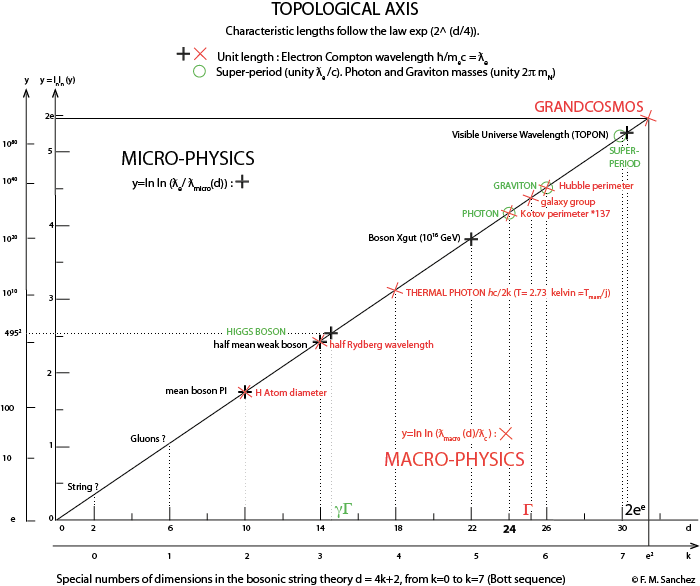
\includegraphics[width=\textwidth,height=14cm]{./figures/figure}
\caption{\textit{The Topological Axis}(data in Table 1). The double natural logarithms (y = lnln(Y)) of the main dimensionless physical quantities (Y) corresponds to the special string dimension series d = 4k + 2, from k = 0 to k = 7, characteristics of the Bott sequence [19]. This is the reunion of height 2D-1D holographic relations, hence the name `Topological Axis`. Two relations comes from the double large number correlation \cite{Eddington}, one comes from the Carr and Rees weak boson-gravitation relation Eq(11)), and one comes from the Davies analysis \cite{Davies}, involving the CMB wavelength. \textit{In the macro-physics side, with length unit $\lambdabar_e$, the Electron Compton reduced wavelength, the Universe circumference} $2\pi \times$ 13.812 billion light-years is tied to the bosonic critical dimension 26, while Bott reduction $\Delta$d = 8 leads firstly to  d = 18: it is the \textit{thermal photon} (Cosmological Microwave Background), tied to the the mammal wavelength through the Sternheimer scale factor $j$ (section 8.2); another Bott reduction leads to d = 10 (super-string dimension): it is the \textit{Hydrogen atom}, and finally to d = 2: the \textit{massive string}, about 2.1 GeV. For the number 24 of transverse dimensions, it is the \textit{Kotov length} (section 4.3), multiplied by a factor about 2$\pi a$, with $a \approx 137.036$. For d $\approx \Gamma$, the Atiyah constant (section 8.2), it is the \textit{galaxy group} radius, a characteristic cosmic length ($10^{6}$ light-years, section 2.1). For k $\approx e^{2}$, $y \approx 2e$, it is the \textit{Grandcosmos} radius (section 3). 
The Space-Time-Matter Holic dimension d = 30 (section 6) is tied to $c$ times the cosmic \textit{Super-period} (section 5). 
\textit{In the micro-physics side, with the same length unit $\lambdabar_e$}, Bott reductions from d = 30 lead to the \textit{gauge bosons}: d = 22 for the GUT one, ($10^{16}$ GeV), d = 14 for the weak one and d = 6 for the (\textit{massive}) gluons, about 8.6 MeV.
For the intermediary superstring value d = 10, there is the mean \textit{Pion}. For d $\approx \gamma \times \Gamma$, Y $\approx 495^2$ the square of the diminushed Green-Schwarz string dimension (496 - 1), it is the \textit{Brout-Englert-Higgs boson} (125.175 GeV). For k $\approx 2e^e$, it is the \textit{topon}, the visible Universe wavelength, the space quantum, which identifies with the mono-radial unit length of the Bekenstein-Hawking Universe entropy (section 3).
   \textit{With unit $2\pi$ times the Nambu mass $m_N~=~137m_e$}\cite{Nambu}, d = 24 and 26 corresponds to the \textit{photon and graviton masses}, defined by two-step holographic interaction \cite{Sanchez1}.}
    \textit{This is the extrapolation toward smaller numbers of the Double Large Number correlation. The central dimension is d = 16, for a total $2^7$ of string dimensions in the Bott sequence. This suggests a liaison with the Eddington's matrix $16\times 16$}\cite{Eddington}.
\label{fig:figure_label}
\end{figure*}

%R\{GC} = 2r_e^6/l_P^5\approx 9.0757\cdot10^{86}m$

\begin{table*}
 \caption{Topological Axis $f(d)~=~exp(2^{d/4})$. Data with $R = 2a_G\lambdabar_e=2\hbar^2/Gm_em_pm_H~ \approx 13.812~ Glyr,R_{GC}=2r_e^6/l_P^5\approx 9.0758\cdot 10^{86}~m $}  
  
  \begin{tabular}{llllll}
    \toprule
    \multicolumn{6}{c}{$\lambdabar_M = 2l_P^2/R \approx 3.9989\cdot10^{-96} m$, $T = \hbar^{4} /\rho_{c}^{3/2} G_{F}^{5/2} \approx 5.4829 \cdot 10^{57} s, l_K = \lambdabar_e(a_Ga_w)^{1/2}, m_{ph}=a_wm_{gr}\approx 1.222\cdot10^{-55}kg$}                   \\
    \cmidrule(r){1-6}
   Physical element     & k     & d = 4k+2 & lnln(f(d)) & lnln(Measured ratio)\cite{Tanabashi} & Predictions~($\lambdabar_e = ar_e = ct_e$) \\
    \midrule
    string & 0  & 2 & 0.347 &  & $ m_{string} \approx$ 2.1~ MeV ~? \\
    gluon  & 1 & 6 & 1.040 &  & $m_{gluon} \approx$ 8.6~ MeV ~? \\  
    mean pion & 2  & 10 & 1.733 & lnln(268.60)$\approx$ 1.722 &  \\ 
    H Atom Diameter & 2  & 10 & 1.733 & lnln(274.22) $\approx$ 1.725  &  \\
    half mean Weak Boson & 3  & 14 & 2.426 & lnln(8.378~$\cdot~10^4)\approx$ 2.428  &   \\
    Higgs Boson & - & $\gamma\Gamma \approx$ 14.533 & 2.518 &lnln(2.449$~\cdot~10^5)\approx$ 2.518& $m_{Higgs} \approx$ 125.175$~ GeV ~$ ? \\ 
    thermal photon & 4  & 18 & 3.119 & lnln($hc/2k\theta_{CMB}\lambdabar_e) \approx$ 3.035 &  \\
    boson GUT & 5  & 22 & 3.812 & & $m_{GUT} \approx 2.30\cdot 10^{16}~GeV~?$ \\
    photon & 5.5  & 24 & 4.159 & & lnln$(m_N/m_{ph})\approx 4.130$ \\
    Kotov perimeter & 5.5  & 24 & 4.159 &lnln($2\pi l_K /r_e)\approx 4.159$ &  \\
    Hubble radius R*6 & 6  & 26 & 4.5054 & 4.506(3)\cite{Bonvin} & lnln$(6 R /\lambdabar_e)\approx$ 4.5054  \\
    graviton & 6  & 26 & 4.505 &  & lnln$(m_N/m_{gr})\approx 4.485$ \\
    Supercycle period & 7  & 30 & 5.199 & & lnln$(T/t_e) \approx$ 5.199 \\
    topon & - & 2$e^e$ & 5.253 &  & lnln$(\lambdabar_e/\lambdabar_M) \approx$ 5.523 \\
    Grandcosmos & $e^2$  & - & 5.432 & & lnln$(R_{GC}/\lambdabar_e)\approx$ 5.433  \\
    \bottomrule
  \end{tabular}
  \label{tab:table}
\end{table*}


\markright{F.M. Sanchez,\ V.A. Kotov,\ M. Grosmann,\ D. Weigel,\ R. Veysseyre,\ C. Bizouard,\ N. Flawisky,\ D. Gayral,\ L. Gueroult, \textit{Back to Cosmos}}
\section {The Cosmic Fine-Tuning and the Topological Axis}
\markright{F.M. Sanchez,\ V.A. Kotov,\ M. Grosmann,\ D. Weigel,\ R. Veysseyre,\ C. Bizouard,\ N. Flawisky,\ D. Gayral,\ L. Gueroult, \textit{Back to Cosmos}}

We look here for a systematic organization of dimensionless physical quantities stemming from cosmology, astrophysics, particle   physics, theoretical physics and mathematics. The most famous fine tuning implies cosmic quantities, awkwardly called the `Double Large Number Problem`. If it is a `problem` for standard evolutionary cosmology, it is a precious clue in the steady-state cosmology based on the \textit{Perfect} Cosmological Principle (spatial \textit{and} temporal homogeneity).
This Cosmological Fine-Tuning leads directly to a \textit{Gravitational Hydrogen molecule model of the visible universe} \cite{Sanchez1}.
This defines the Universe Hubble radius $R = 2a_{G} \lambdabar_{e}$, where the factor 2 comes from the bi-atomic structure, and where $\lambdabar_{e} = \hbar/cm_{e}$ is the Electron Compton reduced wavelength, while the gravitational coupling constant is: $a_{G} = \hbar c/Gm_{p}m_{H}$, where $m_p$ and $m_H$ are the proton and hydrogen atom masses. So, \textit{the speed $c$ is eliminated}, in accordance with the Coherent Cosmology which needs signal celerity far exceeding $c$. This gives $R \approx 13,812~Gly $, corresponding to a Hubble constant 70.790 (km/s)/Megaparsec, compatible with the most recent measurements \cite{Bonvin}: 72(3) (km/s)/Megaparsec. The latter confirms the value measured by the 1a type novae, while the standard optimization of 6 parameters results in a lower value, by $9\%$. This is a significant refutation of the standard cosmology, but the fact that the so-called Universe age is $\approx 13.8~yr$ cannot be due to chance. This means that the standard approch has something right, but the interpretation is false.

Consider the wavelength of the visible Universe with critical mass $M= Rc^2/2G$: 
\begin{equation}
\lambdabar_{M} = \hbar /Mc \approx 4.00 \cdot 10^{-96} m
\end{equation}
This `topon` corresponds to the value $n \approx 2e^e$, close to the touchstone n = 30 of the Topological Axis, see Fig. 1. This scheme illustrates the function $f(n + 4) = f^{2}(n)$
and stems from the imbrication of relations of the form $\lambdabar_{e} /l_{micro} \sim (l_{macro} /\lambdabar_{e})^{2}$, followed by $ l_{macro} /\lambdabar_{e} \sim (\lambdabar_{e} /l^{\prime}_{micro} )^{2}$, leading to:
$$
\begin{array}{ll}
%
\displaystyle
\lambdabar_{e}/\lambdabar_{M} \sim (R/\lambdabar_{e})^{2} \sim (\lambdabar_{e}/ \lambdabar_{X})^{4}\\[+8pt]  % 1st row
\sim (\lambda_{CMB}/ \lambdabar_{e})^{8} \sim (\lambdabar_{e}/\lambdabar_{W})^{16} \sim (2r_{H} /\lambdabar_{e})^{32}\\[+8pt] % 2nd row
\sim (\lambdabar_{e}/ l_{Gl} )^{64} \sim (\lambdabar_{str} /\lambdabar_{e} )^{128} \sim 2^{2^8}\\ % 3rd row
\end{array}
$$
This series include the Cosmic Microwave Background wavelength $\lambda_{CMB}$ and a string wavelength $\lambdabar_{str}$, with mass about 2 MeV. Hence, the correlation is eight-fold. They include implicitly the above double fine-tuning and three  more relations that have been independently reported \cite{Sanchez1}. Thus, only three relations are really new. The overall large number $2^{256}$ has an obvious computational character, confirmed below by the dramatic appearance of the Eddington Large Number.

In particular, as Davies quoted \cite{Davies} \textit{'The fact that $R/\lambda_{CMB}\sim a_G^{3/4}$ seems to indicate yet another large-number coincidence'}. By this order of magnitude, we infer rather precise relations. With the Hydrogen radius $r_H$, we observe 
$ R/r_H \approx (4\pi \lambda_{CMB}/r_H)^{4}$, precise to $0.6\%$. 
Considering the standard cosmological neutrino background (CNB), which wavelength is defined by $(\lambda_{CNB} / \lambda_{CMB})^{3} = 11/4$, we note that $R/ \lambdabar_{e} \approx
( \lambda_{CNB}^{2} / \lambda_{CMB} \lambdabar_{e} )^{4}$ to $1.7\%$. The appearance of the neutrino field is conform with the synthesis of the two main cosmologies, where the single Bang is replaced by a matter-antimatter Oscillatory Bounce \cite{Sanchez2}.

It was noted in \cite{Carr} that $a_{G}$ is of order $W^{8}$, where $W$ is the mass ratio W boson-Electron. With the above $R$ value, one observes the following more symmetrical relation involving the other (neutral) weak boson Z, in the 0.01\% indetermination of $W$ and $Z$:
\begin{equation}
R/(\lambdabar_{p}\lambdabar_{H})^{1/2}\approx (WZ)^4
\end{equation}
where $\lambdabar_{p}$ and $\lambdabar_{H}$ are the Proton and Hydrogen reduced wavelengths. The precision of this formula will be pulled to the ppb range in section 9.4, by intervention of canonical mathematical constants.

The gravitational Hydrogen molecule model \cite{Sanchez1} implies the following double correlation, which is the simplest case of Eddington's statistical theory \cite{Eddington}: the position of a `reference particle` is supposed to be determined 
with an uncertainty of ${R/2}$. 
For N particles of mass $m$ components of the visible Universe, the deviance is statistically divided by $\sqrt{N}$, where $N = M/m$. If $m$ is the principal value of the effective mass of the electron in the Hydrogen atom, $ m = m^{\prime}_{e} = m_{e} m_p/m_H $, and if, moreover, one equates the deviance $R/(2\sqrt{(M/m^{\prime}_{e})})$ to the Hydrogen reduced wavelength $\lambdabar_{H} = \hbar/c m_{H}$, one obtains the double relation:
\begin{equation}
R/2\lambdabar_{H} = (M/m^{\prime}_{e})^{1/2} = \hbar c/G m_{e} m_{p}
\end{equation}
\textit{This is the definitive interpretation of the Double Large Number Fine-tuning}. 
So, while the two pillars of Physics, Relativity and Quantum Theory are unable to conciliate Gravitation 
and Particle Physics, the third pillar, Statistical Physics, directly makes this connection in cosmology \cite{Eddington}.

Recall that, contrary to what is often stated, quantum physics does not limit to micro-physics. Indeed, the exclusion principle applies in both solid state physics and in stellar physics. In particular, for a star containing $N_s$ atoms, in which the pressure has reached the quantum degeneracy value (case of white dwarfs), exclusion principle applies for electrons, and the radius star is about $R/N_{s}^{1/3}$ \cite{Sanchez1}. So the formula giving the Hubble radius $R$, a very difficult measurement which puzzled a whole century, was implicitly contained in astrophysics textbooks. 
The universe radius amazingly appears as the limit of a mono-atomic star radius, for which the electrons are in degeneracy state. Eddingon was aware of this Cosmologic Exclusion Principle, but could not conclude since, at his epoch, the Hubble measurement for $R$ was false by an order of magnitude.

The reason for this discrepancy is that \textit{Lema\^itre and Hubble considered galaxies of the Local Group, which do not participate the so-called space expansion}. In fact, it is sufficient to introduce a repulsive force proportional to separation distance, for explanation of the steady-state exponential recession. \textit{The repulsive force is equivalent to reintroduce  the Einstein cosmological constant, but with invariant value} $1/R^{2}$. There is no need of the so-called `dark energy`.

The distance for which this force exceeds attractive gravitation between galaxies is about $10^{6}$ light years \cite{Sanchez1}, a typical galaxy group radius, which corresponds, in the Topological Axis, to the Atiyah Constant $\Gamma$, (section 8.2), see Fig 1.

In the steady-state cosmology of Bondi, Gold and Hoyle \cite{Sanchez1}, such a repulsive force between galaxy groups is necessary, in order to avoid a big chill due to the thermodynamics second principle. But, inside a galaxy group, another evacuation mechanism must occur: \textit{it would be the role of massive black holes}.

\markright{F.M. Sanchez,\ V.A. Kotov,\ M. Grosmann,\ D. Weigel,\ R. Veysseyre,\ C. Bizouard,\ N. Flawisky,\ D. Gayral,\ L. Gueroult, \textit{Back to Cosmos}}
\section{The Toponic Holographic Quantification}
\markright{F.M. Sanchez,\ V.A. Kotov,\ M. Grosmann,\ D. Weigel,\ R. Veysseyre,\ C. Bizouard,\ N. Flawisky,\ D. Gayral,\ L. Gueroult, \textit{Back to Cosmos}}

In the above steady-state cosmological model, the Perfect Cosmological Principle implies the invariance of the Universe mean mass density $\rho$, defined at large. This predicts also the exponential recession of galaxy groups, with time constant $R/c$ being compensated by the appearance of $m_n$ massive neutrons at rate $c^{3} /Gm_{n}$, 
corresponding to about one neutron by century in about a cathedral volume. 
The invariant visible Universe radius $R$ is then defined by the Schwarszchild relation, so that each topon, with wavelength $\lambdabar_M = \hbar/Mc = 2l_{P}^{2} /R$ is the center of an equivalent $R$-radius black hole, of critical mass $M = Rc^{2} /2G$. The Bekenstein-Hawking entropy of this black-hole Universe shows an 1D extension \cite{Sanchez1} of the standard Holographic Principle, until now devoted to 3D application only \cite{Bousso}:
\begin{equation}
S_{BH} = A/4 = \pi(R/l_{P})^{2} = 2\pi R/\lambdabar_{M}
\end{equation}
where $A$ is the horizon sphere area and $l_{P} = (G\hbar/c^{3} )^{1/2}$ is the Planck's length. Note that, while the standard evolutionary cosmology use differential equations, which are not adapted to a single Universe, as Poincar\'{e} stated \cite{Sanchez1}, the Permanent Cosmology must favor such integral relations. Here it is the \textit{Archimedes Testimony tying the Disk Area to its Perimeter}.

In the standard evolutionary view, the observed homogeneity of causally disconnected regions of space is known as the so-called `horizon problem`, and is at the origin of the awkward inflation hypothesis, which is unnecessary in the steady-state model. Indeed, \textit{the critical condition is provided by the above very definition of $R$}.

The topon breaks the so-called `Planck's wall` by a factor $l_{P}/\lambdabar_{M}\approx 10^{61}$. This explains why this holographic relation was long time unnoticed. Indeed, it was admitted that $l_{P}$ was the quantum of space: in fact \textit{the Planck's length is an intermediate holographic length only}.

The gravitational potential energy of a critical homogeneous sphere is $-(3/5)GM^{2}/R = -
(3/10)Mc^{2}$, while the \textit{non-relativistic} kinetic energy of galaxies is $(3/10)Mc^{2}$ \cite{Sanchez1}. Their sum is therefore zero: the density of the so-called `dark energy` is compatible with 7/10, so that dark energy was a trivial false problem. 
The Relativity theory is a local theory that does not apply in cosmology at large: 
galaxies actually reach speed $c$, and, crossing the horizon, enter a Grandcosmos of radius $R_{GC}$, given, as a first approximation, by the symmetrical holographic relation, here monochrome instead of the above mono-radial one:
\begin{equation}
S_{BH}\, = \pi(R/l_P )^{2} = 2\pi R^{(0)}_{GC} /l_{P}
\end{equation}
with $R^{(0)}_{GC} /R = l_{P} /\lambdabar_{M} \sim 10^{61}$. 
The conservation of the time constant $t = R/c = R^{(0)}_{GC} /C$ introduces a canonical velocity $C \sim 10^{61} c$, 
lifting the veil on an energy larger than that of the visible Universe by a factor of $10^{122}$, which can be identified with the $l_{P}$ - normalized quantum energy of vacuum, checked by the Casimir effect \cite{Duplantier}. The central problem of quantum cosmic physics is thus solved. Moreover, the objections against the Hawking approach using trans-Plankian frequencies are wiped out \cite{Damour}.

In a better approximation, justified below, $R$ is replaced in the above relation by $R^{\prime} = 2\hbar^{2}/Gm_{N}^{3}
\approx 18.105$ Gly, where $m_{N} = am_{e}$ is the Nambu mass, of central importance in particle physics. Indeed, the half radius $R^{\prime}/2$ has a simpler definition than $R/2$: it corresponds to the elimination of $c$ between the classical electron radius and the Planck length \cite{Sanchez1}. In this way, the sphere of radius $R^{\prime}$ appears 
as the spherical hologram representation of the outer Grandcosmos:
\begin{equation}
S^{\prime}_{BH}\, = \pi(R^{\prime}/l_{P})^{2} = 2\pi R_{GC} /l_{P}
\end{equation}
This value will be confirmed in the section 5 (Fig.6).

The Toponic Quantification Hypothesis assumes that the mass of a particle is an exact sub-multiple 
of the critical  mass $M$ of the visible Universe: $m = M/N_{m}$. Thus its wavelength is 
$N_m \lambdabar_{M}$, allowing the following holographic extension of the above mono-radial holographic conservation:
\begin{equation}
S_{BH} = \pi(R/l_{P})^{2} = 2\pi R/\lambdabar_{M} = 2\pi N_{m} R/\lambdabar_{m}
\end{equation}
This series of diametrical circles generate, by scanning, the approximation of a sphere: thus it goes 
from the disk to the sphere with area $4\pi(R/l_{P})^{2}$. Note that \textit{this justifies the factor $\frac{1}{4}$ in the BH entropy}. 
But, for the approximation to be sufficient, \textit{the numbers $N_{m}$ must be very large}. In this way, the Cosmos-
Computer can use the computational properties of the mathematical constants of the continuous analysis, such as $e$ and $\pi$, see section 9 and 10 (Discussion).

The immensity of the Cosmos thus receives a computational holographic explanation, which is much simpler than that of standard cosmology, where initial conditions, during Planck's time, would be adjusted with extreme precision, even with inflation. 

With $N_{Ed} = 136 \cdot2^{256}$ the Eddington's large number, one observes that $N_{Ed}$ times the neutron mass, corrected by the classical ratio $H/p$, gives, to 41 ppm, the effective mass $3M/10$, so that:
\begin{equation}
Mm_p = m_P^4/m_em_H\approx(10N_{Ed}/3)m_Hm_n 
\end{equation}
showing a kind of symmetry between the masses of particles. This directly involves Planck's mass $m_{P}$, which at the present time, has no known interpretation, except that it is close to the mass of the human ovocyte \cite{Sanchez1}. In this way, the local inertia is related to the distant masses, in accordance with the Mach principle, which the relativity theory does not explain. Another shortcoming of this theory is that it does not define any inertial frame. However, the Doppler as-symmetry of the cosmic background indicates that the speed of our local group of galaxies is about 630 km/s. The cosmic background is, therefore, tied to the Newton absolute frame, the Grandcosmos.

The mathematical continuity is excluded by the above Computation Principle, so the time associated to the above 'topon': 
\begin{equation}
t_M = \lambdabar_{M} /c = \hbar/Mc^2 \approx 1.33 \times 10^{-104}s 
\end{equation}
is the new candidate for the `Chronon`, the `quantum of time`, so the Oscillatory Bounce has a frequency about $10^{104}$ Hz  \cite{Sanchez2} and respects the CPT (Charge conjugation-Parity inversion-Time reversal) symmetry \cite{Sanchez1}. note that the tachyonic hypothesis is consistent with the non-local character of quantum mechanics.

\markright{F.M. Sanchez,\ V.A. Kotov,\ M. Grosmann,\ D. Weigel,\ R. Veysseyre,\ C. Bizouard,\ N. Flawisky,\ D. Gayral,\ L. Gueroult, \textit{Back to Cosmos}}
\section{The Tachyonic Flickering Space-Time-Matter}
\markright{F.M. Sanchez,\ V.A. Kotov,\ M. Grosmann,\ D. Weigel,\ R. Veysseyre,\ C. Bizouard,\ N. Flawisky,\ D. Gayral,\ L. Gueroult, \textit{Back to Cosmos}} 

\subsection{The Single Electron Cosmology}

The single-electron cosmology \cite{Sanchez1} uses the electron indeterminacy, which is the real basis of the Exclusion Principle, giving a horizon value $R_1$ only dependent of the principal value of the Hydrogen radius $a^{\prime} = aH/p$, by respect to $\lambdabar_e$. It is the value for which the mean cosmic value is also the atomic one:
\begin{equation}
\frac{\sum(1/n)}{\sum(1/n^{2})} = a^{\prime}
\end{equation}
with the sum running from 2 to $R_{1} /\lambdabar_{e}$. This implies:
$$
R_{1} = \lambdabar_{e} exp((\pi^{2} /6 - 1)a^{\prime} + 1 - \gamma) \approx 15.77465 ~ Gly
$$
very close (0.4 ppm) to $R_{1} = ( p_{G} /p_{0} )(\beta R R^{\prime})^{1/2}$, where $p_{G} = P/2^{127/2}$, with $P = \lambdabar_e / l_P$, $\beta = (H - p)^{-1}$ the Rydbergh correction factor and $p_{0} = 6\pi^{5}$ the Lenz-Wyler value $p$ (Section 9.2). Moreover, there is a direct connection with the Grandcosmos radius and the topon, to 0.90 \%:
\begin{equation}
\lambdabar_M = 2l_p^2/R \approx R_1^3/R_{GC}^2
\end{equation}  
This \textit{synthesis relation} confirms the coherence of the whole procedure. It will be of central importance in the following (section 7.4), where the above lengths $l_P$, $R$, $\lambdabar_M$ and $R_{GC}$ will be connected with $R^{\prime}$, the above holographic reduction length of the Grandcosmos together with the following Kotov length. 

\subsection{The Cosmic Coherent Oscillation (CCO)}

The Kotov non-Doppler cosmic oscillation \cite{Kotov1} is not considered seriously, since it seems to violate the most basic prerequisite of physics, the generality of Doppler phenomena. Interpreting this as a tachyonic phenomenon, we identified the Kotov period $t_{K} \simeq 9600.06(2) s$, taking the electron characteristic time $t_{e} = \lambdabar_{e} /c$ as unit, to the simplest relation eliminating $c$ between $a_{G}$ and $a_{w}=
\hbar^{3} /G_{F} m_{e}^{2} c$, the well measured $(3\cdot 10^{-7})$ dimensionless electroweak coupling constant $a_{w}$ :
\begin{equation}
t_{K} / t_{e} = (a_{G} a_{w})^{1/2}
\end{equation}
This weak coupling constant \cite{Carr} $a_{w} = (E_{F} /m_{e} c^{2} )^{2}$ is defined from the Fermi energy\cite{Tanabashi}: 
$
E_{F} \approx 292.806161(6) GeV \approx 573007.33(25) m_{e} c^{2}
$, itself tied to the weak force constant 
$
G_{F} \equiv (\hbar c)^{3} /E_{F}^{2} \approx
1.4358509(7) \cdot 10^{-62} Joule \cdot m^{3}
$
. This introduces the product of two area speeds, confirming the flickering hypothesis:
\begin{equation}
(\lambdabar_{e}^2/t_{K} )(\hbar/(m_{p} m_{H})^{1/2} = (GG_{F})^{1/2}
\end{equation}
so the best measured cosmic quantity, the Kotov period, implies a symmetry between gravitation and weak nuclear force. This specifies the $G$ valu*e to $10^{-6}$ precision (ppm). It is compatible with the well-elaborate $(10^{-5})$ BIPM measurement \cite{Quinn}, at several sigmas from the Codata value \cite{Tanabashi}, but the later is the mean between discordant measurements. Computer analysis shows that this value of $G$ is compatible with the following well-defined value, with $d_{e} \approx 1.001159652$ the relative electron magnetic moment :
$$\begin{array}{ll}
(2^{127} /a_{G} )^{1/2} \approx d_{e} (H/p)^{3} \\
\qquad  \qquad \Leftrightarrow \\
G \approx 6.6754552 \times 10^{-11} kg^{-1} m^{3} s^{-2} \\
\end{array}$$
This value will be confirmed, in the ppb range, in Section 9.

With the Kotov length $l_{K} = ct_{K}$ (see below), one notes that $(R/a_w l_K)^{1/2} $ is close to $\sqrt{a}$, while the replacement of $R$ by $R_{1}$ is about $4\pi$, the canonical form for $\sqrt{a}$, the deviation being compatible with $p/p_{0}$:
$$\sqrt{(R_{1} /a_{w} l_{K})} \approx 4\pi p/p_{0} \leftrightarrow t_{K} \approx 9 600.591445 s$$ a relation independent from $G$. This $t_K$ value will be confirmed, in the ppb range, in section 9.4. 

From the holographic two-step interaction \cite{Sanchez1}, the Kotov period is associated with the photon mass, a conclusion independently reached by C. Marchal, apart a $2\pi$ factor \cite{Marchal}. It is $m_{ph} = \hbar/c^{2} t_{K} \approx 1.222 \times 10^{-55}$ kg, and the graviton mass is: 
$m_{gr}\, = m_{ph} /a_{w} \approx 3.722 \times 10^{-67} $ kg.
The ratios with $2\pi$ times the Nambu mass corresponds (respectively within 2.9 \% and 3.7 \%)  to the \textit{canonical values} n = 24 and n = 26 (Fig.1). Thus $f(26)/f(24) \approx a_w $ to 0.8 \%. The following relation (0.1\%), will be very usefull in the section 5:
\begin{equation}
M/m_{ph} \approx (3/e)O^2_M
\end{equation}
with $O_M$ the cardinal order of the Monster group.

\subsection{The omnipresence of CC0 in astrophysics}

With $t = R/c$, the relation $(t t_{K}^2)^{1/3} \approx 10.8$ years, compatible with the famous 11 years sun period was noted. It was proposed that this unexplained phenomenon, responsible for moderate periodic climate variation, was also of flickering cosmic origin \cite{Sanchez3}. This hypothesis has been recently confirmed by the straight temporal profile of the phenomena, showing it is tied to a quantum process \cite{Kotov2}.

Remarkable enough, a `mysterious` period $\approx 1/9$ days of the Sun's pulsations has been predicted long before its actual discovery in 1974. Namely, 73 years ago, French amateur astronomer Sevin (1946) claimed that « la p\'{e}riode propre de vibration du Soleil, c'est-a-dire la p\'{e}riode de son infra-son (1/9 de jour), a jou\'{e} un role essentiel dans la distribution des plan\`{e}tes sup\'{e}rieures». Presumably, the Sevin's «vibration period» of the Sun was merely an issue of his reflections about resonances and distances inside the solar system. Nevertheless, solar pulsations with exactly that period were discovered, after decades, - and independently of the Sevin's paper, - by a few groups of astrophysicists. Soon the presence of the same period, or timescale, was found in other objects of Cosmos too \cite{Kotov1}.

Opponents emphasize often that $t_{K}$ is very close to the 9th harmonic of the mean terrestrial day: the corresponding ratio - of the length of a day to the $t_{K}$ period - is equal to 8.99943(1), - and claim thus the $t_{K}$ oscillation of the Sun should be regarded as an artifact (see, e.g., Grec and Fossat, 1979; Fossat et al., 2017). As a matter of fact, however, the $t_{K}$ period occurs to be the best commensurate timescale for the spin rates of all the most massive and fast-rotating bodies of the solar system, in general.

\begin{figure}
\centering
\includegraphics[width=7cm,height=5.5cm]{./figures/figure1}
\caption{Resonance-spectrum $F(\nu)$ computed for 15 motions of the largest, fast-spinning bodies of the solar system. On horizontal axis is logarithm of frequency $\nu$ in $\mu$Hz, the dashed horizontal line shows a $ 3 \theta $ C.L., and the primary peak yields to the best - commensurable period 9594(65) s.}
\label{fig:figure_label}
\end{figure}

\begin{figure}
\centering
\includegraphics[width=7cm,height=5.5cm]{./figures/figure2}
\caption{Same as Fig. 2, for N = 11 sizes `diameters` of the solar system (with c = 1 and the $\pi$ factor for inner orbits). The highest peak corresponds to the spatial scale 9600(120) light sec.}
\label{fig:figure_label}
\end{figure}

This is obvious from Fig. 2, which shows the resonance spectrum $F( \nu )$, calculated for 15 motions of 12 largest, fast spinning, objects of the system (with the mean diameters $\geq 500$ km and periods inferior to 2 days: six planets, three asteroids and three satellites, leaving apart trans-neptunian objects; see Kotov, 2018). The peak of the best commensurability corresponds to a period of 9594(65) s, which coincides well, within the error limits, with $t_K$ at about $5.3 \theta$ C.L., i.e. with a chance probability $10^{-7}$.

It seems very puzzling also that the spatial scale $l_{K} \approx 19.24$ A.U. occurs to be the best commensurate with orbital sizes of the main planetary orbits of the solar system, - see Fig. 3, where the resonance spectrum $F( \nu )$ is plotted for 11 orbits, including those of asteroid belt, Pluto and Eris (orbital «diameters» were approximated by the major axes, and for the inner orbits they were multiplied by $\pi$). The primary peak - of the best commensurability - corresponds to the spatial scale 9600(120) light sec., or 19.24(3) A.U., at $4.7 \theta$ C.L. (Kotov, 2013).



\begin{figure}
\centering
\includegraphics[width=7cm,height=5.5cm]{./figures/figure3}
\caption{Resonance-spectrum $F_{1} ( \nu)$, computed for N = 5746 binaries with periods inferior to 5 days. Horizontal axis gives logarithm of the trial frequency $\nu$ in $\mu Hz$, the dashed line indicates a $3 \theta$ C.L., and the major peak corresponds to a timescale of 9590(70) s.}
\label{fig:figure_label}
\end{figure}


Close binaries are characterized by the $t_{K}$ resonance too, with the $\pi$ number as a factor of ideal incommensurability of motions, or frequencies (Kotov, 2018). Fig. 4 shows the resonance spectrum, or metrics of motion, $F_{1} (\nu) \equiv F(\pi \cdot \nu/2)$, computed for 5746 close binaries, including cataclysmic variables and related objects. The major peak, with C.L. of about $7 \theta$, corresponds to the timescale 9590(70) s, coinciding within the error limits with $t_{K}$ (the stellar data were taken from all available binary stars catalogues and original papers).

To compute the $F_{1} (\nu)$ spectrum, the program finds - for each test frequency $\nu$ - deviations of ratios $(2\nu_{i} /\pi \nu) k \geq 1$ from the nearest integers, and determines then the least-square minimum of such deviations. Here, $\nu$ is the test frequency, $\nu_{i}$ minus the frequency of a given object, i = 1, 2, ...N - the ordinal number, with N, the total number of observed periods in a sample of objects, and the power k = 1 or -1. The factor of two in Eq. (2) takes into account that second half of the orbit repeats the first one, and the transcendental number $\pi$ appears as a factor of orbital stability, or «ideal» incommensurability, of motions, or frequencies (the $\pi$ number, in fact, characterizes geometry of space; for details see Kotov, 2018).

Recently it was shown, that the $t_K$ timescale characterizes, statistically, the motion of superfast exoplanets too, see Figure 5.

It was shown in fact, that a number of superfast, with periods inferior to 2 days, exoplanets revolve around parent stars with periods, near-commensurate with timescales $t_{1}$ and/or $2 t_{1}/\pi$, where $t_{1} = 9603(85) s$ agrees fairly well with the period $t_{K} \approx 9600$ s of the so-called «cosmic oscillation», found firstly in the Sun, then - in other variable objects of the Universe (the probability that the two timescales would coincide by chance is near $3 \cdot 10^{-4}$).

\begin{figure}
\centering
\includegraphics[width=7cm,height=5.5cm]{./figures/figure4}
\caption{Same as Fig. 4, for the $F_{2} ( \nu )$ spectrum, computed for N = 145 exoplanets with P inferior to 1.5 days. The strongest peak of the composite commensurability corresponds to a period of 9640(115) s, at nearly $3.9\theta$ significance (after Kotov, 2018).}
\label{fig:figure_label}
\end{figure}

\subsection{The Tifft, Arp and Pioneer effects}

Another unexplained effect is the 75(5) km/s periodicity in the galactic redshift \cite{Tifft}. Now, this speed corresponds to the quantum resonance: $$ v_{n} = N v_{1} = N \hbar /r_{e} m_{F} $$ where $r_{e} = \lambdabar_e/a$ is the electron classical radius and $m_{F} = m_{e}\sqrt{a_{w}}$ is the Fermi mass.

The Halton Arp observations of chains of galaxies with different redshifts \cite{Arp} was also rejected. But it could be the sign of the galactic regeneration constantly maintaining the visible Universe mass: this is sustained by the following section proving the invariance of the mean mass density $\rho_{c}$.

Much controversial is the Pioneer deceleration \cite{Nieto} $g_{Pi} \approx 8.7 \times 10^{-10} ms^{-2}$. It corresponds to he Pioneer time $t_{Pi} = c/g_{Pi} \approx 3.4 \times 10^{17} s $ close to $t = R/c \approx 4.3587 \times 10^{17} s $. The following section will show a connection between the Kotov, Tifft and Pioneer effects.

\markright{F.M. Sanchez,\ V.A. Kotov,\ M. Grosmann,\ D. Weigel,\ R. Veysseyre,\ C. Bizouard,\ N. Flawisky,\ D. Gayral,\ L. Gueroult, \textit{Back to Cosmos}}
\section{The Logic of Prospective Dimensional Analysis}\markright{F.M. Sanchez,\ V.A. Kotov,\ M. Grosmann,\ D. Weigel,\ R. Veysseyre,\ C. Bizouard,\ N. Flawisky,\ D. Gayral,\ L. Gueroult, \textit{Back to Cosmos}}

Physics use principally \textit{physical quantities} of the type $Q = M^{x} L^{y} T^{t}$, where $M$, $L$ and $T$ are Mass, Length and Time measurements, and where the exponents are rational numbers. However, the addition of measures of different categories has no significance. This seems at first sight illogical since, fundamentally, a product is a sum of additions. So, \textit{there must be a hidden common nature for the three categories, mass, length and time}. This sustains the above single electron cosmic model \cite{Sanchez1}. 

This suggests a 3D geometrical model. Indeed, consider $t =R/c$, and $M^{\prime} = R^{\prime} c^{2} /2G$ the critical mass in the above holographic sphere representing the Grandcosmos. Summing the square of $ln(M^{\prime}/m_{e} )$, and two times the square of $ln(R/\lambdabar_{e} ) = ln(t/t_{e} )$, one gets, to 40 ppm:
\begin{equation}
ln^{2} (M^{\prime}/m_{e} ) + ln^{2} (R/\lambdabar_{e}) + ln^2 (t/t_{e} ) \approx ln^2 (R_{GC} /\lambdabar_{e} )
\end{equation} 
\textit{showing the Grandcosmos}. This traduces, in function of $P = m_P/m_e$ by:
\begin{equation}
ln^2(P^4/a^3) + 2 ln^2(P^2/pH) \approx ln^2(2P^5/a^6)
\end{equation}
Moreover, to $10^{-7}$, corresponding to $7 \times 10^{-6}$ precision on the above G value:
\begin{equation}
ln^2(P^4/a^3) + 2 ln^2(P^2/pH) \approx exp(4e – 1/a)
\end{equation}
 
This is a dramatic geometrical confirmation (Fig. 6) of the visible Universe – Grandcosmos holographic couple, confirming in paricular the B.I.P.M. measurement of $G$ \cite{Quinn}.


\begin{figure}[h]
\centering
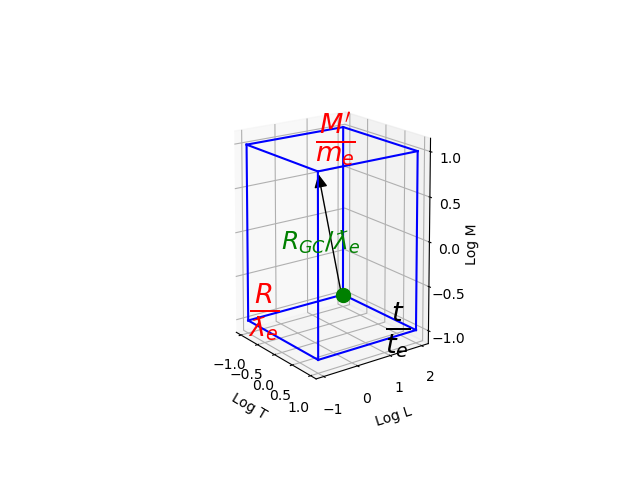
\includegraphics[width=5cm,height=6cm]{./figures/triaxis.png}
\caption {\textit{Geo-dimensional Universe-Grandcosmos couple}, with unit length the Electron Compton reduced wavelength. 
In a 3D Super-space, logarithms of physical ratios are considered vectors. The Grandcosmos radius appears as the norm of the vector using for length and time projections the same value $R/\lambdabar_e$.
%that of the Hubble radius, and for mass ratio $M^{\prime}/m_e$.
$M^{\prime}$ being the critical mass in the Grandcosmos reduced spherical hologram, this is a dramatic geometrical confirmation of the Extended (2D-1D) Holographic Principle applied to the Bekenstein-Hawking Universe entropy. The Grandcosmos existence cannot be denied since the relation involving \textit{natural} logarithms with $e$ and $a$ reach precision $10^{-7}$.} 
\end{figure}

Another crucial point in Physics is the existence of invariant fundamental constants. Thus, association of three of them must give characteristic values of $M$, $L$, $T$. So, approaching a domain in Physics necessitates to calculate characteristic values ($M, L, T$) from the three universal constants which are the most pertinent in the considered domain. This Prospective Dimensional Analysis is largely used in Fluid Mechanics, where the equations are intractable. However, it is largely ignored in other domains because there is not really mathematical foundation, apart the above essential remarks. The triplet $c, G, \hbar$ which define the above Planck units is a notable exception. However, there is no standard interpretation for the Planck mass. Note that  it appears above (Eq. 7) and in Biology \cite{Sanchez1}. 

\textit{Indeed, in virtue of the above Hierarchy Principle, the lack of theoretical justification is not a reason to neglect Prospective Dimensional Analysis}. 

The elimination of $c$ in the above $R$ formula means that the simplest basic dimensional
analysis starting from $\hbar$, $G$ and $m$, the Electron-Proton-Neutron mean mass, gives a good
approximation for $R/2$. Indeed, in the Hypothesis of a coherent Cosmos, it is logical to discard $c$
which is far two small a speed. This has not been observed during one century since $c$ is always
believed to be the single mandatory foundation of space-time. The warning of Poincar\'{e}, the true
discoverer of Relativity: \textit{`use 4D space-time, but do not confound Space and Time`} has long been
forgotten, and physicists have unwisely put $c = 1$ in their equations.

In his three first minutes of cosmology (sept.1997), the first author obtained the length:
\begin{equation}
l \{\hbar,G,m\} = \hbar^{2} /Gm^{3} \approx R/2
\end{equation}
but it took nine years to get this published \cite{Sanchez3}, and it appeared later \cite{Sanchez1} that $m$ must be considered more precisely as the cubic root of the product 
$ m_{e} \cdot m_{p} \cdot m_{H}$. Moreover, the above critical condition
links the time $t = R/c$ and the mean mass density by the $c$-free formula:
\begin{equation}
\rho_{c} = 3/8\pi Gt^{2} \approx 9.41198 \times 10^{-27} kg \cdot m^{-3}
\end{equation}
Thus, the mainstream idea of a temporal variability of the mean density $\rho_{c}$ cannot be to
sustain, meaning that $\rho_{c}$ must be considered a fundamental constant. This writes:
\begin{equation}
t\{\hbar,\rho_{c} ,G\}\, = 1/\rho_{c}^{1/2} G^{1/2} = (R/c) (8\pi/3)^{1/2}.
\end{equation}
This idea of $\rho_{c}$ being a fundamental constant permits to define $R$ without any ambiguity: this is the 
radius of the sphere containing a critical mass. This justifies the above application of the Bekenstein-Hawking entropy. 

Opponents would say that the
center of a black hole presents a singularity: that is indeed the case for the topon in the above flickering Space-
Mass-Time hypothesis. Other will argue that the flying galaxies cannot reach the celerity $c$ at
horizon, but, as recalled above, Relativity is a local theory, so do not apply to cosmology at large.
Indeed, even General Relativity in unable to define any Galilean frame, while the Foucault
pendulus shows it directly, realizing the Cosmic Microwave Background frame, identified with the
Grandcosmos frame, as seen above.

Introducing the Fermi constant $G_{F}$, the associated $c$-free length is very particular, to $1.7\%$:
$$l\{\hbar,\rho_{c},G_{F}\} = \hbar/\rho_{c}^{1/2} G_{F}^{1/2} \approx 9.07154 \times 10^{9} m \approx \lambdabar_{e}^{2}/l_{P}$$
Now, most dramatically, the following mandatory $c$-free times are close to each over $(0.7\%)$:
\begin{equation}
T\{\hbar,\rho_{c} ,G_{F} \}\, = \hbar^{4} /\rho_{c}^{3/2} G_{F}^{5/2} \approx 5.4829 \cdot 10^{57} s
\end{equation}
\begin{equation}
T^{\prime}\{\hbar,G,m\} = \hbar^{3} /G^{2} m^{5} \approx 5.5224 \times 10^{57} s
\end{equation}
One would conceive it as the periodic time of a Super-cycle, which matches the Topological Axis at n = 30,
the holic dimension (see section 6), to 4\%. Comparing $T$ with the Kotov Non-Doppler Cosmic
Oscillation period $t_{K} \approx 9600.60(2)$ s, one observes, to 0.04 \% and 0.2 \%:
$$T/t_{K} \approx O_{M} /\sqrt{2} \approx e^a / \sqrt{a_w} $$
where $O_{M}$, the cardinal order of the Monster Group, have been detected in the section 4.2, again in relation with the Kotov period. Eliminating the later, this introduces the above $t_M$ chronon :
\begin{equation}
T/t_M \approx (3/e\sqrt{2})O_M^3
\end{equation}
The simplest interpretation follows: \textit{this is the number of quantum events in a Super-cycle of period $T$, in a perfectly deterministic Cosmos}. 

The  Monster  Group,  the largest of 26 sporadic groups, is suspected by some researchers to play a central role in Physics: indeed string theory allows a bridge between apparently no-connected mathematical theories \cite{Borcherds}. See below the dramatic properties of $O_M^3$ and $O_M^9$.

Introducing the above Pioneer abnormal deceleration $g_{Pn}$, one gets the time: 
$
t\{G, m_{e} , g_{Pn} \} = (Gm_{e} /g_{Pn}^{3} )^{1/4} = (t_{Pn}^{3} t^{\prime}_{e} )^{1/4}
$, where $t_{Pn} = c/g_{PN}$ and $t^{\prime}_{e} = Gm_{e} /c^{3}$ . This time is compatible with:
$
t\{G, m_{e} , g_{Pn} \} = t_{K} /(F/a)^{2}
$, where the above Tifft factor $F/a$ appears. The implication of the time 
$t^{\prime}_{e}\, = Gm_{e} /c^{3} = 2.2568 \times 10^{-66} s$
confirms the above Planck's wall breakdown.

\markright{F.M. Sanchez,\ V.A. Kotov,\ M. Grosmann,\ D. Weigel,\ R. Veysseyre,\ C. Bizouard,\ N. Flawisky,\ D. Gayral,\ L. Gueroult, \textit{Back to Cosmos}}
\section{The Arithmetical Logic: Holic Principle}
\markright{F.M. Sanchez,\ V.A. Kotov,\ M. Grosmann,\ D. Weigel,\ R. Veysseyre,\ C. Bizouard,\ N. Flawisky,\ D. Gayral,\ L. Gueroult, \textit{Back to Cosmos}}

In the hypothesis of an Arithmetical Cosmos, the ultimate equations must be diophantine. The
simplest one is $T^{2} = L^{3}$, where $T$ is a time ratio and $L$ a length one, resolved, since 2 and 3 are 
co-prime, by:
\begin{equation}
T^{2} = L^{3} = n^{6}
\end{equation}
where n is a whole number, showing the classical 6D phase-space of point mechanics. Considering the exponents, this particularizes the usual 3D space, but attributes 2 dimensions for the Time, in conformity with an independent study \cite{Bars}.

\textit{This is the degenerate arithmetic form of the 2D-3D holographic principle}.

This is \textit{also} the third Kepler's law. It was the simplest one of his three laws, and the realization of his research of harmony. Indeed, its Diophantine form says more: it gives $L = n^{2}$, \textit{the orbit law in the Hydrogen atom and in our Gravitational Molecule model}, where the visible Universe corresponds only to the first orbital. This suggests at once the existence of a Grandcosmos. 

Before the super-period was reckognized, the first version of the Topological axis \cite{Sanchez1} showed an overall dis-symmetry. This was another sign for the Grandcosmos existence.   Now, this corresponds to d = 30, the natural extension of the above Diophantine equation:
\begin{equation}
T^{2} = L^{3} = M^{5} = n^{30}
\end{equation}
where $M$ is a mass ratio. Recall that the lifetime of an unstable particle depends on the $5^{th}$ power of its mass. This holic dimension 30 is the touchstone of the Topological axis, from which the gauge bosons are deduced by Bott reductions [19] (Fig. 1).

This is called the Holic Principle, but limited to \textit{the apparent MLT world only}. The Complete Holic
Principle \cite{Sanchez4} involves a field term $F^{7}$, and so introduces the dimension $30 \times 7 = 210$. This is confirmed by (to 15 ppm, 1.1 ppm, 56 ppm):

\begin{equation}
R/\lambdabar_{e} \approx s_4^5 \approx f(26)/6 \approx \Gamma^{28}/5 \approx (2/\delta)^{210}
\end{equation}
where $s_4 = 2\pi^2 a^3$ is the area of the 4-sphere of radius $a$ and $\Gamma$, the Atiyah constant (section 8.3). Moreover (0.1 \%, 0.03 \% and 0.9 \%):
\begin{equation}
2/\delta = 2R/R^{\prime} \approx lnp/lna \approx lna/ln\Gamma \approx ln\Gamma/lnf
\end{equation}
where $f$ is the inverse strong coupling constant (section 8.3). This  confirms the central computational role of $\delta = R^{\prime}/R = pH/a^{3}$, which is to 1.6 ppm: $\delta \approx e^{2/e^2}$. This implies a geo-combinatorial relation between $a$ and $p$:
\begin{equation}
 p^{(p^{2})} \sim (a^{2})^{(a^{3})}   
\end{equation}
showing a symmetry between basic powers of $a$ and $p$. The consequences of the appearance of $\Gamma$\ in the above equation will appear in section 8.3. 












\markright{F.M. Sanchez,\ V.A. Kotov,\ M. Grosmann,\ D. Weigel,\ R. Veysseyre,\ C. Bizouard,\ N. Flawisky,\ D. Gayral,\ L. Gueroult, \textit{Back to Cosmos}}
\section{The special holographic relations}
\markright{F.M. Sanchez,\ V.A. Kotov,\ M. Grosmann,\ D. Weigel,\ R. Veysseyre,\ C. Bizouard,\ N. Flawisky,\ D. Gayral,\ L. Gueroult, \textit{Back to Cosmos}}

The holographic technique, based on the properties of a coherent wave, is by far the most efficient way to treat huge information, in particular in optics \cite{Grosmann}. Now, the main lesson of modern physics is that everything (light \textit{and} matter) propagates by waves (quanta appearing only at the detection). Moreover, a coherent wave is represented by a unitary operator: we have shown that the quantum formalism is very similar to the holographic one, describing an interaction by a two-step holographic process. From these considerations and CCO study, the masses of the photon and graviton has been proposed (section 4.2).

The students of the first author realized in 1987 a hologram by scanning a 1 mW security power laser beam upon a photo-sensible area of $0.6~ m^2$. The emulsion depth 10 microns permitted false color to be obtained by varying illumination through a photo-mask, and use of a shrinkable emulsion chemical process. The information contained in this hologram reached $10^{15}$ bit, obtained in 12 minutes of scanning exposition. Then, the first author claimed \textit{'such an efficient way of dealing information must be used by Nature'}. Turning to the impressive data of Particle Physics, after an intensive study, holographic relations were indeed found, and its arithmetical form, the Holic Principle was presented at ANPA 16 (Cambridge, 1994) \cite{Sanchez4}. 

In Sept. 1997, the Orsay University attributes a sabbatical year, giving time to reexamine the foundation of cosmology. \textit{In the three first minutes, the half-radius of visible Universe was obtained}. After several weeks, the scanning holography of section 3 was established. After rejection by the Orsay university and Paris Academy, this was put in March 1998 in a closed draft in the Acad\'{e}mie des Sciences de Paris, under the title \textit{ 'L'Univers conserve-t-il l-information ?'}.

Strangely enough, when the first author's publication was blocked (1993-1995), a Holographic Principle was coined by some theoreticians \cite{Bousso}, which were not specialists holography. The origin of this appellation is not clear. One may think that the name comes from the idea of dimension reduction, from 3D to 2D, similar to the visual impression in current visible holograms (in fact holography is only the 2D restitution of a propagating wave). It this respect, it is strange that no one tried to extend this process to 1D. The idea of temporal 1D holography was proposed in the first author's thesis as soon as 1975. 

While the standard Holographic Principle is limited to using the Plank area, it is natural to suppose that they are other holographic units. In fact, \textit{the Topological Axis is the reunion of eight 1D-2D holographic relations}. We present here three more confirmations. 

\subsection{The Conservation of Information}

The Grandcosmos holographic reduction radius $R^{\prime}$ shows itself an holographic
relation with the CMB Wien wavelength $l_{CMB} = hc/kTv $, with $v = 5 (1-e^{-v}) \approx 4.965114245)$ (to $0.01\%$):
\begin{equation}
4\pi(R^{\prime}/l_{CMB})^{2} \approx e^{a}
\end{equation}
Since the holographic technique uses coherent radiation, this seems incompatible with the CMB
thermal character. But \textit{in a totally deterministic cosmos, there is no paradox}. This question is
connected with the black hole information paradigm \cite{Preskill}. Independently of our approach, an
argument in favor of a total conservation of information was tied to a non-evolution cosmology
\cite{Nikolic}. 

Note that \textit{$e^{a}$ is also compatible with the half volume of the proton, with
the Planck length as unit}.

So, while General Relativity and Quantum physics disagree about the nature of Space-Time, especially the non-locality phenomena, they agree for complete determinism, leading to \textit{the definitive rejection of the
Copenhagen statistical interpretation}. 

The Wien wavelength enters (0.03 \%):
\begin{equation}
l_{CMB} / \lambdabar_e \approx P/pH a^3
\end{equation}
confirming that the cosmic temperature is invariant. 

\subsection{The Cosmic Temperature}

In the gravitational hydrogen molecule model \cite{Sanchez1}, $R$ is defined by the following 1D-2D Special
Holographic Relation, using the wavelengths of the electron, proton and hydrogen, while the background wavelength appears in the logical extension, the 3D term involving the molecular Hydrogen wavelength:
\begin{equation}
2 \pi R/\lambdabar_{e} = 4 \pi \lambdabar_{p} \lambdabar_{H} /l_{P}^2 \simeq (4\pi/3)(\lambdabar_{CMB} /\lambdabar_{H2})^{3}
\end{equation}
The above relation gives $T_{CMB} \approx 2.73 K$. With the measured temperature of the cosmic
background, there is a small gap compatible with $(H/p_G)^2 p/6\pi^5 $, where $p_{G}^{2} = P^{2} /2^{127}$ , with $P = \lambdabar_{e} /l_{P}$. 
This eliminates $l_{P}$, producing a relation independent of $G$, implying $T_{CMB} \approx 2.725820805$ Kelvin. Recall
that $2^{127} - 1$ is the most famous prime number in the history of Mathematics, being the last term of
the Combinatorial Hierarchy \cite{Sanchez1} of special imbricated Mersenne numbers 3, 7, 127, the sum of which is 137 (section 8.2):
\begin{equation}
2^{2^{{2^{2^2 - 1}-1}}-1}-1 = 2\pi^{2} \lambda_{CMB}^{3} /\lambdabar_{e} \lambdabar_{H}^2   
\end{equation}
which is the area of the 4-sphere of radius $\lambda_{CMB} / \lambdabar_{m}$, where $\lambdabar_{m} = (\lambdabar_{e} \lambdabar_{H}^2)^{1/3} $. This proves the relevance of
the Lenz-Wyler approximation for the Proton/Electron mass ratio $p_0 = 6\pi^{5}$, (section 9.2). 
%\begin{equation}
%2^{2^{{2^{2^2 - 1}-1}}-1}-1
%\end{equation}

\subsection{The Holic Principle and CCO}

The sphere of radius $R^{\prime} = 2r_e^3 / l_P^ 2$, where $r_e = \lambdabar_e /a $ is the electron classical radius is the Grandcosmos hologram (section 3). Its HB entropy writes: $\pi (R^{\prime}/l_P)^2 = (\pi /2)(R^{\prime}/r_e)^3 $, i.e. with a wrong geometric coefficient. However, the HB entropy of the visible Universe shows a nearly geometric term, with imprecision $\sqrt{4/3\delta} \approx 1.17$:
\begin{equation}
\pi(R/l_P)^2 \approx (2\pi/3)(R/r_e)^3 
\end{equation}
which is a holographic conservation in \textit{the half-sphere of the visible universe}. By analogy with the above scanning process filling the whole sphere (section 3), the above Kotov length $l_k$ (section 4.3) permits to introduce two holographic relations, involving the whole sphere (0.90 \% and 2.6 \%):
\begin{equation}
\pi(R/l_K)^2 \approx 2\pi l_K/r_e 
\end{equation}
\begin{equation}
(4\pi/3)(R/l_K)^3 \approx 4\pi (r_e/l_P)^2 
\end{equation}
The deviation of the first relation is very close to that of the relation $R_1^3 \approx R_{GC}^2 \lambdabar_M$ inducing, to 17 ppm (identified in Eq. () as $np^2/H^2\sqrt{pH}$ to 0.3 ppm) and 0.1\%: 
\begin{equation}
 (R_{GC}l_P/Rr_e)^2 \approx (R_1l_K/Rr_e)^3 \approx \mu^{35}/ln2
\end{equation}
showing a holic form, involving the Muon/Electron mass ratio $\mu$ (see section 9.5).
Taking account of the identity: $2l_P^2 = \lambdabar_M R = (R^{\prime}r_e)^3/(R_{GC}l_P)^2$, this leads to:  (above 17 ppm and 1.8 ppm) :
\begin{equation}
r_e/\lambdabar_M \approx (R_1l_K/R^{\prime}r_e)^3 \approx (4\pi P/p_K)^4
\approx (5/4)^2 \mu ^{35} \end{equation}
with the Koide-Sanchez constant $p_K$, characteristic of the two heavy leptons (section 9.5).
The above term $R_1l_K/R^{\prime}r_e$ is close to (1\%) $\sqrt{O_M} \approx 2a^2P$ (0.18 \%). The study of deviations shows the intermediate bosons ratios $W$ and $Z$, with values specified to the ppb range in section 9.4, leading to (-4 and 3.5 ppm, 0.3\%):
\begin{equation}
O_M (FR^{\prime}/PR_1)^2 \approx W^4 (137/a)^3
\end{equation}
\begin{equation}
 (F^3R_1 / 2 a^3R^{\prime})^2 \approx Z^4 (a/137)(p_0/p)^2
\end{equation}
This precises the relation $a_w/WZ \approx \sqrt{a}$ known (0.1 \%) in Particle Theory (0.3 and -0.4 ppm)
\begin{equation}
137 p_0 W^2 Z^2/p a_w^2 \approx \sqrt{O_M}/(2a^2 P) \approx e^{-4a}
\end{equation}   
Thus, in first approximation $(e^{-1/4a} \approx ~0.036 ~\%)$, the square root of the Monster order is the ratio of the Rydbergh wavelength to the Planck length.







\markright{F.M. Sanchez,\ V.A. Kotov,\ M. Grosmann,\ D. Weigel,\ R. Veysseyre,\ C. Bizouard,\ N. Flawisky,\ D. Gayral,\ L. Gueroult, \textit{Back to Cosmos}}
\section{The role of Intermediary Mathematical Constants}
\markright{F.M. Sanchez,\ V.A. Kotov,\ M. Grosmann,\ D. Weigel,\ R. Veysseyre,\ C. Bizouard,\ N. Flawisky,\ D. Gayral,\ L. Gueroult, \textit{Back to Cosmos}}

\subsection{The electrical constant $a$}
The electrical constant $a$ characterizes the Coulomb force between two $l$-distant elementary charges at rest:
\begin{equation}
F_{qq} =\hbar c/al^{2}    
\end{equation}
Since any electrical charge is a whole multiple of unitary charge $q$ (a relativistic invariant), \textit{any electrical force depends only of the above constants and whole numbers}. Hence, it is logical that $a$ appears central in Atomic Physics and in many fine-tuning relations \cite{Carr}.

However, theorists focused on one property only, the appearance of its fifth power in the Hydrogen hyper-fine spectra, calling its inverse $\alpha$, the `fine-structure constant'. 

Many researchers looked for the mathematical origin of $a$. In quantum electrodynamics, $\sqrt{a}$ is connected with the Electron magnetic abnormal factor, which is very precisely measured\cite{Tanabashi}: $$d_e \approx 1.00115965218076(27)$$
It is readily seen that $\sqrt{a} \approx exp(\pi /2)^2$. From $i = e^{(i\pi /2)}$, this writes $i^{-lni}$ and the study of deviation leads to, with $a_e = a/d_e$ (29 ppb):
\begin{equation}
i^{-lni}/\sqrt{d_e} \approx (\sqrt{a_e} + 1/\sqrt{a_e})^2    
\end{equation}
The slight deviation is not a valid objection, since \textit{Nature must use rational approximations for} $\pi$. Indeed, the fractional development for the corresponding $\pi$ value is 3,7,15,1,$(\tau/\mu)^2$, with $\mu$ and $\tau$ the normalised masses of the heavy leptons.

The standard model is unable to explain the three families of particles. Thus, the study of the muon and tau mass ratios is crucial. One observes (1 ppm, 56 ppm, 0.06 \%):
\begin{equation}
2/\delta \approx (1/2d_{e}) ln(pH)/lna \approx (1/d_e^{2})ln\tau/ln\mu\approx d_e^2 lns/ln\tau
\end{equation}
where $s$ is the Higgs ratio (Section 9).
The following Koide relation \cite{Koide}, \textit{ which has a mathematical justification in term of circulant matrix} \cite{Brannen}, correctly predicted $\tau$ at an epoch (around 2000) during which its measurement was false to 3 $\sigma$. It writes:
\begin{equation}
(1 + \mu + \tau)/2 = (1 + \sqrt\mu + \sqrt\tau)^2/3 = p_K
\end{equation}
This Koide relation, quite discarded by the scientific community, is another sign of the serious incompleteness of the present Particle Physics standard.
This Koide-Sanchez constant, $p_K \approx 1842.604994$, was detected in Eq. (), leading to (2 and 0.16 ppm):
\begin{equation}
p_K^4 \approx (4\pi)^4 apH \approx (pH)^2 137a/136(a^{\prime}-1) d_e
\end{equation}
with $a^{\prime} = r_H/\lambdabar_e = aH/p$. The pertinence of the numbers 136 and 137 is shown in the following.


\subsection{The Eddington's constant 137}

The initial Eddington's proposal for $a$ was the whole number 136, being the number of independent parameters in the symmetric matrix $16 \times 16$. Note that \textit{n = 16 is the central dimension of the Topological Axis}. Later, one unity was added, becoming 137\cite{Eddington}. It shows a symmetry between the 11 dimensions of M theory (a synthesis of five string theories) and the 4 of space-time. Indeed: $137 = 11^{2} + 4^{2}$, while, as seen above: $11/4 = (\theta_{CMB}/\theta_{CNB})^{3}$.

Since Riemann series are tied to the prime number distribution, it seems odd and incredible that mathematicians
have not point out the primes appearing in the harmonic series since it is the single Riemann pole. It seems
that the basic precept \textit{all occurs in the pole} was forgotten in this case. 

As ancient Egyptians used only fractions of type $1/n$, they were certainly aware of this particular harmonic series: 
$S_{5} = 137/60$. Indeed it appears in the Ptolemaic approximation for $\pi$: $\pi_{Pt} = 377/120 = 2 +  S_{5}/2$.

It is strange that Eddington's Theory was rejected as soon as $a$ appeared to deviate from 137. Indeed, the
following shows that \textit{137 plays a central role in ppb fine-tuning analysis}. Note that Nambu \cite{Nambu} showed that the mass $ m_N = 137m_e $ is central in particle physics.


One may interpret 137 + 1 as
the sum of the numbers of dimensions in the Topological Axis \cite{Sanchez1}, taking into account the double
point (H atom-Pion couple) for the super-string value d = 10, and the remarkable sum:
\begin{equation}
\sum_{k=7}^{k=0}(4 k + 2) = 2^{7}
\end{equation}
So $137 = 2^{7} - 1 + 3 + 7$, i.e. the Combinatorial Hierarchy form \cite{Sanchez1}. But this appears also as 137 = 135 + 2, showing the string dimension 2. Indeed, one obtains the value $a \approx 137.035999119$
compatible with measurement value in:
\begin{equation}
ln137/ln(a/137) \approx (2+135/d_{e})^{2}
\end{equation}
meaning that \textit{the ratio $a/137$ acts as a canonical ratio}. 

Considering the product of the T.A. dimensions:
\begin{equation}
P_d = \Pi_{k=7}^{k=0}(4 k + 2) = g_{Suz}/2^73^45^27^111^113^1
\end{equation}
which is a simple sub-multiple of the cardinal order of the Suzuki group, and a simple multiple of the three other sporadic groups $M_{11}, M_{12}$ and $J_2$ \cite{Aschbacher}.
With $l_W$ the mean of the CMB and CNB Wien lengths (0.06 \%):
\begin{equation}
P_d \approx l_W / \lambda_e
\end{equation}
The pertinence of the T.A. series is thus confirmed, calling for further study.

\subsection{The Atiyah and Sternheimer constants}
    Sir Michael Atiyah was a precursor in the search for unity in Mathematics and Physics. 
In his last work \cite{Atiyah1} the Bernoulli function $x/(1-e^{-x})$ plays a central role. \textit{This is the kernel of the thermal Planck law}. Considering the above Wien reduced constant $v = hc/kT\lambda_{Wien}$, one notes that $a \approx e^v -2\pi$, suggesting $a$ to be a trigonometric line. Indeed $cosa \approx 1/e$, and, to 65 ppb:
\begin{equation}
a \approx 44\pi - Arccos(1/e)
\end{equation}
a formula diffused on the web, but without indication of its connection with the Planck law.
Moreover, $v$ appears in the normalised neutron mass $n\approx 1838.6836089(17)$ (13 ppb):
\begin{equation}
n^{1/3}\approx v~(\pi/2)^2  
\end{equation}
The small deviation is again attributed to a rationalisation of $\pi$: 3,7,16,-(1+$\tau/\mu)^2$.

Another central constant in the Planck law is the irrational Apery constant $\xi(3) \approx 1.20205691$. The number of photons in a sphere of radius $r$ is:
$n_{ph}(r) = (4\pi/3) (r/l_{ph})^3$
with $l_{ph} = (hc/k_B \theta) (16\pi \xi(3))^{-1/3}$. The photon density is $l_{ph}^{-3} \approx $ 410.872 photons/$cm^3$. The standard value is 410.7(4) ~ $cm^{-3}$  \cite{Tanabashi}. 

The critical photon/baryon ratio is $ \eta_{cr} = n_{ph}(R) m_n/M$. While the number of photons exceeds the baryon number, it is the contrary for the energy densities, which is, for the CMB alone $u_{CMB} = (\pi^2/15)\hbar c /\lambdabar_{CMB}^4$. However, the energy density of the sum CMB and CNB is the later times $1 + 3 \times (7/8) (4/11)^{4/3} \approx 1.681321953$, to be compared to $u_{cr} = \rho_{cr} c^2$. One notes the dramatic relation between these two canonical ratios, with the 2 factor coming from photon polarisation (0.4 \%): 
\begin{equation}
\sqrt{2\eta_{cr}} \approx \frac{u_{cr}}{u_{CMB + CNB}} 
\end{equation}
This is an Eddington type relation, confirming that they are only three neutrinos, and ruining again the standard \textit{evolutionary} cosmology.
%Moreover, $2\eta_{cr}$ is connected to the above Suzuki group order by $g_{Suz}/2 \eta_{cr} \approx e^w \sqrt{p} \approx (10/3) p$, to 0.3 \% and 0.2 \%. This confirms the implication of the sporadic groups, and the value of the ratio critical/real baryon number about $\sqrt{p}/2$\cite{Sanchez1}. 
Moreover (0.08 \%):
\begin{equation}
E = l_{ph}^{(CMB)}/\lambdabar_e \approx (\pi a^2)^2
\end{equation}
This term is central in the unification number \cite{Sanchez4} (0.07 \%):
\begin{equation}
U = \Phi^{137} \approx (1-e^{-v})^{-1}~ (\pi a^2)^6 
\end{equation}
We recall that this quasi-whole number, based on the golden number $\Phi$, shows a holic character\cite{Sanchez4} (0.03, 1, 0.07 \%, 43 ppm, 0.4 \%)  :
\begin{equation}
U  \approx (\pi P/Dp_K)^2 \approx E^3 \approx (pH/2a)^7 \approx (\tau^2/\mu^3)^{210} \sqrt{\delta}
\end{equation}
with $D = 196883$ the Monster Moonshine dimension\cite{Conway}.
    
Atiyah introduced also the constant 
\begin{equation}
 \Gamma = \gamma a /\pi
\end{equation}    
as a simplification term. One observes: 
\begin{equation}
2/\delta = 2a^3/pH \approx (1/2d_{e}) ln(pH)/lna \approx lna/ln\Gamma
\end{equation}
With  $w = F/W$, this leads to (22 ppm):
\begin{equation}
a/\Gamma = \pi /\gamma  \approx w^{\delta}
\end{equation}
while, with $z = F/Z$ (3 ppm):
\begin{equation}
 137/\Gamma \approx z^{\sqrt{f}/2}   
\end{equation}
where $f$ is the Bizouard strong constant precising the inverse 8.44(5) of the standard 'strong coupling constant'\cite{Tanabashi}:
\begin{equation}
f = a_w/2\pi (pH)^{3/2} \approx 8.43450
\end{equation}
Since $wz\approx \sqrt{a}$ \textit{this seems to be at the kernel of the Particle standard model}, calling for further study. 

In cosmology, $\Gamma$ and the canonical $e^{\pi}$ enter the following dramatic simplification of the above (Section 4.1) single-electron cosmic formula (0.3 ppm):    
\begin{equation}
a^{\prime} = ((ln(R_1/\lambdabar_e) + \gamma – 1)/(\pi^2/6 - 1)) \approx ln(R/\lambdabar e) + \Gamma + e^{\pi}
\end{equation}
so confirming the $R$ value to 45 ppm.

Moreover, this confirms the role of $j = 8\pi^2/ln2$, the Sternheimer scale factor\cite{Sanchez1}  (to 0.013 \%, 0.013 \%, 0.046 \%):
\begin{equation}
j \approx ln(R/\lambdabar e) + \Gamma \approx a - e^{\pi} \approx e^{\pi} lna
\end{equation}
The Titts group order $13\cdot 2^{11}3^35^2$ \cite{Titts}  completes the biophysics relations involving central temperatures \cite{Sanchez1}: 
\begin{equation}
j\approx T_{mam}/T_{CMB} \approx O_T / W
\end{equation}
\begin{equation}
10^2\approx T_{H_2O}/T_{CMB} \approx O_T / Z
\end{equation}
The pertinence of $O_T$ is confirmed by the 2 ppb relation, where 71 is the biggest prime in the Monster order: 
\begin{equation}
2\times 137^2 + 21 = 23^2\times 71 \approx 3\times 137 d_e O_T/D    
\end{equation}


The mammal wavelength enters (1\%)
\begin{equation}
(Rl_P)^{1/2}\approx hc/kT_{mam}
\end{equation}
It is known that the reduced series $8k^{\prime}+2$ gives for $k^{\prime}$ = 1 and 3 the canonical values 10 and 26. Now the value $k^{\prime}$ = 2, d = 18 is at last interpreted: \textit{the couple thermal photon-Life is at the upper center of the Topological Axis}, while the down center is the Higgs boson (Fig.1). The real center, as seen above, is the dimension d = 16. Moreover, to 0.1\%, the water triple point enters (0.1 and 1 \%):
\begin{equation}
(R^{\prime}l_P)^{1/2}\approx hc/k\theta_{H_2O}
\end{equation}
\begin{equation}
\theta_{H_2}\times \theta_{O_2} \approx \theta_{H_2O} \times \theta_{CMB} 
\end{equation}
This shows that Chemistry is also involved \cite{Sanchez1}.

The study of the 22 amino-acids \cite{Sanchez1} has shown that $j$ is also a computation base. Indeed, to 2\%: $j^{22} \approx 3 P^2 $ and, more precisely, to 0.01 \% :$j^{22} \approx Pp_E^7 $ where $ p_E \approx 1847.599459$ is the Eddington's mass ratio of the couple proton-electron, the roots ratio in the Eddington's equation $10x^2 - 136x + 1 = 0 $.



\subsection{The ubiquity of $a^{a}$}
\markright{F.M. Sanchez,\ V.A. Kotov,\ M. Grosmann,\ D. Weigel,\ R. Veysseyre,\ C. Bizouard,\ N. Flawisky,\ D. Gayral,\ L. Gueroult, \textit{Back to Cosmos}}

Since 137 is a number of parameters, it must be interpreted as a dimension i.e. a privileged exponent. However, from the Computation Hypothesis, $a$ must be an optimal base also. \textit{So the term $a^a$ must be central}.
    
Indeed, apart a $\pi$ factor, $a^a$ is the Grandcosmos volume with unit length the Hydrogen radius, to 0.4 and 0.5 \%:
\begin{equation}
(4\pi/3)(R_{GC}/r_H)^3 \approx a^a/\pi \approx 3(1/ln2)^{\sqrt{pH}}
\end{equation}
\textit{Note that the ln2 factor involves the information theory}. This relation is tied to the following property of the above Unification factor (0.06 and 0.1 \%):
\begin{equation}
U = \Phi^{137}\approx a^{p/a}\approx (1/ln2)^{pn/137^2}
\end{equation}
Moreover, the dramatic relation $a^a\approx e^{p/e}$ has been connected with the fifth optimal musical scale (306 notes) and to the operational definition of $e$ \cite{Sanchez1}. Hence,  we look here for its manifestations in classical mathematics. 

The famous Lucas-Lehmer primality test uses the series of whole numbers $N_{n+1} = N_{n}^{2}-2$,
starting from $N = 4 = u_{3} + 1/u_{3}$, with $u_{3} = \sqrt{3} + 2$. The later is a special case of Diophantine generators $u_{n} = \sqrt{n} + \sqrt{(n+1)}$, whose entire powers are close to whole numbers. One shows that $N_{n} \approx u_{3}^{(2^{n})}$, and for n = 9:
\begin{equation}
u_{3}^{(2^9)} \approx (2(137^{2} + 48))^{64} \approx a^{a}
\end{equation}
defining $a$ to 39 ppm and showing that the Rydbergh term $2a^2$ plays a central role.

Also, with the Pell-Fermat generator $u_{1}
 = 1 + \sqrt{2}$:
\begin{equation}
a^{a} \approx u_1^{3\times(2^{8}-1)}
\end{equation}
which defines $a$ to 0.3 ppm. So the number $a$ establishes a connection between $u_{1}$ and $u_{3}$, two of the
simplest arithmetic's generators. This opens a \textit{new research in pure mathematics}. %Remark that the $12^{th}$ Pell-Fermat number is $ u_1^{12}/2 \approx 140^2 + 1 \approx a(a+6)$ to 4 ppm. 



\subsection{The intervention of Sporadic Groups}

One observes, to 30 ppm, 0.5 \% and 0.05 \%:
\begin{equation}
O_{M} \approx  (lnlnlnO_{M})^{2(136 + d_e)} \approx (\pi/2)^{2a^{\prime}d_e^2} \approx (F/af)^{20}
\end{equation}
Moreover (0.036 \% and 0.038 \%):
\begin{equation}
O_{M}^{1/10} \approx 495^2 \approx f(\gamma \Gamma) 
\end{equation}
where $495 = g_0/16$, implying the order $g_0$ of the smallest  sporadic group (Mattieu) order $M_{11}$. Note that 495 is a unity less than the Green-Schwarz string dimension 496, the third perfect number, after 6 and 28. The precision 1.7 ppm of $f(\gamma \Gamma)\approx 495^2 (a/137) $ suggests that the Higgs ratio is $495^2$,
 corresponding to 125.175 GeV (Fig 1 and Table 1).
 %Also, in the Topological Axis (Fig. 1), it corresponds with $k \approx \pi $, and n $\approx \gamma \Gamma \approx (4\pi + 2) (p/d_e p_0)^2$, to 30 ppb.

The product of the 6 pariah group orders verifies (7 ppm):
\begin{equation}
\Pi_{pariah} \approx (F/a)^{20}/d_e^2
\end{equation}
thus, the above cosmic Tifft ratio $F/a$ (section 4.4) is directly tied to the six pariah groups. This establishes a connection between the six pariah groups and the Monster group (0.7 \%):
\begin{equation}
\Pi_{pariah}/O_M\approx f^{20}
\end{equation}
These six pariah groups are not identified to form any family. By contrast, the 20 normal sporadic groups form the so-called \textit {happy family} which is closely related to the Monster. The product of the 20 groups of the happy family shows, to 0.015\%, 1\% and 0.45 \%:
\begin{equation}
\Pi_{happy} \approx \delta \cdot a^{a} \approx (j/495)^2~ \Gamma^{210}
\end{equation}
where $j/495$ is close to the weak mixing angle 0.23116(12) \cite{Tanabashi}, to 0.45 \%. This confirms the above Complete Holic Principle, and the computation role of $\Gamma$. Moreover, to 2\%: $a^a \approx \Gamma^{209}$. From the order of the Baby-Monster $O_B\approx\Gamma^{24}$, and $209 = 137 + 3\times 24$ (1 and 2 \%):
\begin{equation}
O_B \approx \Gamma^{24} \approx  (a/\Gamma)^{a/3}
\end{equation}
 where $a/\Gamma = \pi/\gamma $ is the above canonical Atiyah ratio. 

The total product of the 26 sporadic orders $\Pi_{26}$ verifies (0.27 \%):
\begin{equation}
\Pi_{26} \approx (9/2)(R_{GC}/\lambdabar_M )^2
\end{equation}
Now $\Pi_{26}$ is close to the holic term $e^{4 \times 210}$, whose $a^{th}$ root is very remarkable (65ppm, 98 ppm, 5 ppb):
\begin{equation}
e^{4 \times 210/a} \approx 2e^{2e} \approx H/4 \approx 26 \times (2 \times 26 + 1)/3
\end{equation}
The ppb range precision of the last term means clearly that a rationalization of $e^{2e}$ is occurring, where the canonical dimension 26 plays a central role.

Note that $p/g_0$ is close to the above weak mixing angle (0.3 \%. This ratios appears as calculation base in the product of cardinal orders of the Monster and the baby-Monster groups, to 1\%, 0.2 \%, and 1 \%:
\begin{equation}
O_MO_B\approx H^{2H/a} \approx (g_0/p)^a \approx (496/j)^{137}
\end{equation}
confirming the central role of the weak mixing angle.  The photon number in the visible universe is (0.1 \% and 0.2 \%):
\begin{equation}
n_{ph} \approx (3/\pi)~ e^{e^6/2} \approx \sqrt{\delta}~ O_M O_B
\end{equation}
With $N_{ph}$ the photon number in the Grandcosmos, and $N_n = M_{GC}/m_n$ the equivalent neutron number in the Grandcosmos, one observes (3 \%, 0.5 \%):
\begin{equation}
\sqrt{N_{ph}N_n} \approx e^{n/3} \approx (O_M^3/U)^2  
\end{equation}
confirming that the Grandcosmos is the external thermostat of the visible Universe. This is tied to (3 \%, 0.08\%, 2.5\%,1\%):
\begin{equation}
e^{137e}\approx Ue^{n/6}\approx (e/3)e^{ea}\approx O_M^3 \approx 496^{60} 
\end{equation}
With the tachyonic ratio $V = R_{GC}/R = C/c$, the orders of the two giant sporadic groups enter (0.2 \%, 0.1 \% and 79 ppm):
\begin{equation}
V \approx 44 \pi N_{S} \approx (a/\pi) O_M D \approx (a/\pi) O_B P a^{3/2}
\end{equation}
where $N_S = 2^{65} \cdot 3^{41} \cdot 5^{28}$ is the Systema number\cite{Moulin}.

The corrected Eddington's number $N_{Ed}^{\prime} = a \cdot 2^{256}$, where 136 is replaced by $a$, shows (4.5 ppm and 0.03 \%):
\begin{equation}
N_{Ed}^{\prime} \approx 6 \cdot 137PO_M \approx (3/4) a p a_w (V/O_M)^9
\end{equation}

With the 4D area $ s_4 = 2\pi^2 a^3$, the holic reduction  
\begin{equation}
(R/\lambdabar_e)^7 \approx (3/2) O_M^5 \approx s_4^{35} 
\end{equation}
implies $O_M^{1/7} \approx s_a^{(4)}$. Indeed, the Monster appears to be close to the seventh power of the pariah group $J_3$ (0.2 ppm): 
\begin{equation}
O_M \approx d_e J_3^7 \sqrt{p/p_0}
\end{equation}
\textit{The above relations proves that physics establish unexpected bridges between sporadic groups, including the Titts one}.

With $\delta_K = p_K^2/a^3 $, and the symetrised Planck area $(l_P^{\prime})^2 = \sqrt{h \hbar} G/c^3$ (11, -11 ppm, and 0.04 \%):
\begin{equation}
(1/2\pi^{3/2})(R_{GC}/l_P^{\prime})^4 \approx (\delta_K O_M )^9 e^{1/2a} \approx  \mu^{210}/4\pi \approx \tau^{137}
\end{equation}
The existence of a Final Theory based on the Holic Principle (section 6), the Grandcosmos and the Koide-Sanchez constant cannot be denied. The interpretation is clear: \textit{the 4D space-time of Grandcosmos is associated with a 9D space involving the Monster. This opens a path towards the Final Theory}

\markright{F.M. Sanchez,\ V.A. Kotov,\ M. Grosmann,\ D. Weigel,\ R. Veysseyre,\ C. Bizouard,\ N. Flawisky,\ D. Gayral,\ L. Gueroult, \textit{Back to Cosmos}}
\section{The fine-tuning with basic mathematical constants}
\markright{F.M.Sanchez,\ V.A.Kotov,\ M.Grosmann,\ D.Weigel,\ R.Veysseyre,\ C.Bizouard,\ N.Flawisky,\ D.Gayral,\ L.Gueroult,\ Back to Cosmos}
\markright{F.M. Sanchez,\ V.A. Kotov,\ M. Grosmann,\ D. Weigel,\ R. Veysseyre,\ C. Bizouard,\ N. Flawisky,\ D. Gayral,\ L. Gueroult, \textit{Back to Cosmos}}

We look here for relations involving basic mathematical constants, noting firstly that, to 6.5 ppm:
$p \approx \Gamma (\pi e)^2$. 

\subsection {The optimal calculation base $e$ confirmed}

The electron magnetic moment $2d_e$ appears in (0.7 ppm):
\begin{equation}
a/\Gamma = \pi/\gamma \approx 2d_e \cdot e ~(p_0/p)^2 
\end{equation}
The Topological Axis shows clearly that the Grandcosmos is defined by the following conjunction (1\%):
\begin{equation}
f(k = e^{2}) = exp(2^{e^{2+1/2}}) \approx exp(e^{2e}+e^{2})
\end{equation}
where the supplementary term $exp(e^2)$ is close to $a^{3/2}$. Note the following properties of the 'economic number' $e^{e^e}$, to 
0.4 \%, 6 ppm and 0.8 ppm:
\begin{equation}
e^{e^e}\approx (lnp)^{lnp} \approx 137 (e^{e})^3 \approx e^e a \sqrt{pH} (p/p_0)^2 
\end{equation}
With $a_1 = a-1$ (8 ppm, 0.2 ppm, and 0.05 \%):
\begin{equation}
e^{e^e}/a_1^2 \approx 4 ln P \approx a ln(9/2) \approx 5^{2^7}
\end{equation}
showing the role of musical bases 2, 3 and 5. Note that the Topological Axis terminal term $e^2$ is the limit of the following musical series:
$$(3/2)^5 \approx (4/3)^7   \approx (5/4)^9  \approx  (6/5)^{11}  \approx   ...  \approx  (1+1/n)^{2n+1}  $$  
a series converging much rapidly than the classical $(1+1/n)^n$. The first two terms defines the occidental 12 tones scale.
Note that, to 0.6 \% and 0.03 \%:
\begin{equation}
R/\lambdabar_e \approx 2^{2^7}
\end{equation}
\begin{equation}
R^{\prime}/\lambdabar_e \approx (3^3)^{(3^3)}
\end{equation}

The canonical ratio $R_{GC}/\lambdabar_M = 2P^9/a^6pH $ confirms the Full Holographic Principle, to 0.04 \%:
\begin{equation}
R_{GC}/\lambdabar_M  \approx (137e/a)^{2 \cdot 210}  
\end{equation}
exhibiting (0.3 ppm): $ (a/137)^{420} \approx (137 - 3)/120 $  
with $137 - 3 = 7 + 127$ showing the Combinatorial Hierarchy terms\cite{Sanchez1}. 


\subsection {The Lenz-Wyler's Formula}
Wyler published a value approaching $a$ to 0.6 ppm and confirmed the pertinence of the Lenz approximation which plays a central role above: $p_{0} = 6\pi^{5} \approx p$ to 18.824 ppm.

The Lenz-Wyler formula is the product of the area by the volume of a 3D cube with side $\pi$. If one considers a 3D cube with side 5, privileging again the identification dimension = exponent, this gives $6 \times 5^5 = 137^2 - 19 $. This is not a chance coincidence because this relation has long time been deduced from basic considerations on quarks \cite{Sanchez1}. Indeed with $u = 5 $ and $d = 6 $, the combination $uud = 150 $, whose power 3/2 is close to $H$, while the combination $udd \approx (n/a)^2 $ shows the neutron/electron mass ratio $n$. This leads to (0.012 \%) $6\times 5^5 \approx (aH/n)^2 $.  
Note that, with $q = 2^{12}$ to 0.03 \%, 2.5 \% and 41 ppm:
$$R_{GC}/\lambdabar_e \approx q\times 5^{137} \approx 6^{137}/q^2 \approx 6^{128}/(1+1/\sqrt2)$$
Since $R/\lambdabar_e \approx 2^{128}$, \textit{ 
the factorisation of 6 leads to a natural Universe- Grandcosmos partition}, and to the following approximation for the tachyonic celerity ratio (0.01\%) 
$$ U = C/c\approx3^{128} (p_K/p_G \delta)^2 $$ where $p_K$ is the Koide-Sanchez constant (see section 9.5). This confirms the role of the correspondence quark up = 5 and \textit{quark d = 6 with a double structure}. This elimination of $q$ leads to (2.6 \%):
$(R_{GC}/\lambdabar_e)^3 \approx (uud)^{137}$. 

It is an example of \textit{immergence}, i.e. deducing the small from the large, in a striking similitude between cosmology and nuclear physics. Another example was encountered in section 2.4, where dimensional analysis gives the visible Universe radius, in an easier way than the equivalent one for the Hydrogen atom radius, since for this case there is no evidence that $c$ must be left out. Another example signals a general misconception: the coherence of the stimulated emission in a laser is a \textit{global effect} in a homogeneous media (atomic coherence). 

\subsection {The Archimedes constant $\pi$ as a calculation base}
\markright{F.M. Sanchez,\ V.A. Kotov,\ M. Grosmann,\ D. Weigel,\ R. Veysseyre,\ C. Bizouard,\ N. Flawisky,\ D. Gayral,\ L. Gueroult,\textit{Back to Cosmos}}

The value of the Topological Function for the main String
 dimension 26 renders, to 0.1\%, the same Lenz-Wyler form $f(26) \approx 6(2\pi^{2} a^{3} )^{5}$, where $2\pi^{2}a^{3}$ is the area of a 4-sphere of radius $a$. Moreover, with $n/p$ the mass ratio Neutron/Proton, to 0/3\%, 0.02\% and 1ppm:
\begin{equation} 
(p/n) (R/\lambdabar_{e})^{2} \approx (f(26)/6)^{2} \approx (2\pi^{2} a^{3})^{10} \approx \pi^{155}
\end{equation}
The corresponding approximation $\pi_R$ of $\pi$ shows the fractional series 3, 7, 16, -u, with $u \approx
2 \times 137$, confirming again the Rationalization Hypothesis of section 3. This leads to the rational value
$\pi_{R} = (355u-22)/(113u-7)$. This corresponds to the above $G$ value to 10 ppb accuracy.
Since $(R/\lambdabar_{e})^{2} \approx 2^{256} $, this illustrates the following musical relation involving again 137: $2^{1/155} \approx \pi^{1/256} \approx (2\pi)^{1/3 \times 137}$. The scale with 155 notes is not known, but 137 appears also in the classical musical scales \cite{Sanchez1}. Whole powers of $\pi$ appears in the even order Riemann series, and in:
$a \approx 4\pi^{3} + \pi^{2} + \pi $ (Reilly formula, 2 ppm), while $a \approx \pi^{9/2}2^{-1/3}$ (8 ppm). Moreover, with $P = \lambdabar_e/ l_P$ (0.3 and 0.07 \%):
\begin{equation}
P^3 \approx \pi^{a-2} \approx (2\pi R/\lambdabar_e)(2 \pi l_K/r_e) 
\end{equation}
confirming the Planck volume and the Kotov length.


\subsection {The Four Forces Connection in ppb Fine-Tuning}

The Particle standard model achieved the unification between electromagnetism and weak nuclear force, with extension to strong nuclear force in the Grand Unification Theory (GUT), but without any synthesis with gravitational force. However, the Topological Axis shows clearly that GUT with $1O^{16}$ GeV gauge boson seems confirmed. Very precisely, in section 4.2, it is proven that the CCO oscillation reveals a symmetry between the electroweak and gravitational forces. So we look here for a precise relation involving the 4 force parameters, $a$ (electric), $a_w$ (weak nuclear), $f$ (strong nuclear) and $a_G$ (gravitation). The later force is equivalently represented by $p_G = P/2^{127/2}$, with $P = m_P/m_e$. 

 With the Atiyah constant $\Gamma = \gamma a/\pi$ (section 8.2), inside the 0.5 ppm measurement precision:  
 $a_{w} = F^2 = (137 \times 2 \Gamma)^{3}$. Now $a_{w}$ is a cube: $a_{w} = (\lambdabar_{e}/l_{eF})^{3}$, with $l_{eF} = (G_{F}/m_{e} c^{2})^{1/3}$:    
\begin{equation}
\lambdabar_e/l_{eF} \approx 137 \times 2\Gamma
\end{equation}
leading to $F = a_{w}^{1/2} = E_{F} /m_{e} c^{2} \approx 573007.3652$. Moreover:
\begin{equation}
aF/\sqrt(pH) = 2\pi afpH/F \approx \pi(4n/\Gamma)^3/p_G \approx \mu^2
\end{equation}
where $\mu$ is the Muon/Electron mass ratio, \textit{inside its 20 ppb undetermination}, so proposing the value:
\begin{equation}
\mu \approx 206.7682869
\end{equation}
Note that $4n/\Gamma$ is close (3.4 ppm) to the monstrous $5^{th}$ term 292.6345909 in
the fractional development of $\pi$ which is itself very close to $n/2\pi$ to 3.4 ppm. Since the fractional
development of $\pi$ is to this date an unsolved problem, \textit{this confirms that current mathematics is
incomplete and that Nature uses rational approximations of $\pi$}.

These relations show a dual form, the first one without any numerical factor:
\begin{equation}
ap_{G} / \pi \sqrt(pH) \approx (n F/137^{2} \Gamma^{3} )^{3} \approx (4n/ \Gamma)^{3}/F
\end{equation}
Now,
 as was recalled above, the exponents represent the number of
dimensions. So, this represents a dimensional reduction, eliminating 137, from 9D and 6D to
3D, which could be associated with the super-string theory, where the equations are coherent only if space
has 9 dimensions, and if the 6 supplementary dimensions unfold on very small distances \cite{Polchinski}.


The following weak boson ratios $W$ and $Z$ match (Eq.1):
$R/\sqrt(\lambdabar_{p} \lambdabar_{H} ) \approx (WZ)^{4}$
\textit{in the ppb range}: 
\begin{equation}
W \approx 137^{2} \Gamma / 3d_{e}
\end{equation}
\begin{equation}
Z \approx ap^{2} \pi^{4} / 137 d_{e} n
\end{equation}
\textit{The ultimate theory must explain these ppb relations.}


\markright{F.M. Sanchez,\ V.A. Kotov,\ M. Grosmann,\ D. Weigel,\ R. Veysseyre,\ C. Bizouard,\ N. Flawisky,\ D. Gayral,\ L. Gueroult, \textit{Back to Cosmos}}
\section {Discussion}
\markright{F.M. Sanchez,\ V.A. Kotov,\ M. Grosmann,\ D. Weigel,\ R. Veysseyre,\ C. Bizouard,\ N. Flawisky,\ D. Gayral,\ L. Gueroult, \textit{Back to Cosmos}}

For many, cosmology is the hardiest chapter of physics. This modern, negative, opinion is in fact in contrast with the ancient culture, for which \textit{the cosmology is the first of all sciences, so must be the simplest}. In the original meaning of the word `revolution`, it is a return to the source of Science, the `all is whole number` of Pythagoras. Even the degenerate form of topological or holographic relations, the simplest diophantine equations, the Holic Principle, shows direct pertinence. In particular, it emphasizes the 30 dimensions, which appear decisive in the Topological Axis, and are identified with the sum of 26 string dimensions and 4 of usual space-time.

The distinction between Length and Time must be emphasized, as
Poincar\'{e}, the father of 4D Relativity Theory recommended. Indeed their confusion, by writing $c$ =
1, impeded the fact that the Hubble-Lema\^{i}tre radius $R$ is a trivial length, directly given by the prospective $c$-free dimensional analysis, which gives also the cosmic temperature and the cosmic super-cycle period.

This means also that the International System must go back to only three fundamental unities,
Mass, Length and Time.

The Hierarchy and Computation principles presented in section 1 are confirmed both by the Topological axis, the geo-dimensional Universe-Grandcosmos Couple, and the mononomial relations (i.e. merely products of parameters). These accurate mononomial relations reunifies Mathematics and Physics. The precision reaches the ppb domain: they cannot be due to chance. This shows how the so-called 'free parameters' are misnamed: they are imposed by Nature proving the Cosmos Unicity. As Atiyah wrote \cite{Atiyah1}: \textit{`Nobody has ever wondered what the Universe would be if $\pi$ were not equal to 3.14159.... Similarly no one should be worried what the Universe would be if $a$ were not 137.035999...}` This is a \textit{definite refutation} of the Multiverse Hypothesis. In this respect, the high precision in the measurement of the Electric and Fermi constants, Proton, Neutron and Muon masses, Kotov cosmic period, and, with lesser precision, the background temperature, must be saluted as decisive achievements.

The pertinence of these simple mononomial relations cannot be admitted by the standard community, arguing for instance that since the proton is composite, its mass cannot enter simple relations. The same argument is presented for the theoretical dependence of the electric constant $a$ with other constants, or with the energy level. These are reductionist arguments, unable to explain the fine-tuning phenomena, and leading to the sterile concept of unexplained emergences. By contrast, the holistic approach implies the concept of \textit{immergence}, resulting from the ancestral idea that Cosmos simplicity is the real origin of Science. It is strange, revealing and troubling that this term \textit{immergence} is a neologism.

The Cosmos concept has long been forgotten. This is the reason why quantum physics is not really understood. Indeed, the simple fact that the propagation of anything, light or matter, is wavy, while the reception is a quantum, was a central mystery along the last century. This simple fact induces non-locality, so the necessary intervention of cosmology. Moreover, the optimal utilisation of the wavy propagation is holography, whose formalism is similar to the quantum one. Thus it is logical to find holographic relations in cosmology. Moreover, the similitude between the formalisms of quantum physics and holography is so tight that the double-step holography is similar to the double step of any interaction: tachyonic propagation - non-local cosmic optimisation - local quantum reception.

Thus tachyonic-holography physics is necessary. Hence, it was an error to reject the bosonic string theory under the pretext it involves tachyons \cite{Woigt}. Quite the contrary, it is an essential advantage. This is confirmed by the central importance of the bosonic dimension d = 26 in the Topological Axis, which is nothing that the extension to smaller numbers of the Double Large Number coincidence, that only Eddington interpreted correctly, by rejecting the Single Bang model. Many invoked the temporal variation of the parameters, which is a negation of the idea that physics have universal laws. Finally, the expedient of the Anthropic Principle was imposed to the community by some leaders: this is definitely refuted in this article.

Moreover, the standard Holographic Principle must be generalized to wavelengths others than the Planck
length, in particular the topon, the visible Universe wavelength, in 1D holography, which breaks by an enormous factor, about $10^{61}$ a taboo of current thinking: the Planck wall, resolving the vacuum energy dilemma factor $10^{122}$, and sustaining the Oscillatory bounce model which unfies the two main cosmologies.

This leads back to the main hypothesis of this article: the Cosmos is a computer, and the dimensionless parameters are calculation bases. A common point with the brain is precisely this \textit{multi-base} character, experienced in musical sensation. It is no chance that the parameters are encountered in the musical scales and DNA chain. Thus, Intelligent Life receives a justification: to help the cosmological computation. This Inverted Anthropic Principle answers the first of all questions: \textit{why one asks question ?} 

Thus, \textit{intelligent life must be universal}. The famous Fermi question `where are they ?` is not a paradox, since any abnormal observation is \textit{a-priori} rejected by a dogmatic community. This destroy the Darwin `accidental life` approach, a generally admitted so-called `theory` with too much missing links \cite{Chauvin}.

The same rejection seems to apply now to the Sternheimer 'scale wave' and Atiyah's last work. The present article shows that at least parts of these works are very pertinent. This follows the rejection (with the notable exception of Schrodinger) of Eddington\cite{Eddington} himself. Only Eddington interpreted rightly the Cosmic Large Number correlations, as recalled in this article. While he dared to apply the exclusion principle in cosmology, it is the basis of our Single Electron Cosmologic model (section 4.1) which rehabilitates once more his work. Also, fortunately, the large theoretical advance of Eddington is now recognized \cite{Durham}, but without mentioning a crucial point: \textit{he predicted the tau fermion with a right order of mass}, 30 years before its surprising discovery, calling it Heavy Mesotron \cite{Eddington}. Moreover, it seems that no one realizes that the Eddington prediction for the baryon number in the visible Universe is so accurate. Note that many mocked the Eddington Large Number, not to speak of his number 137, completely rehabilitated by the monomonial relations.

However, curiously, Eddington believed in the standard statistical interpretation. Thus, he did not reached the above conclusions. Also, at his epoch the holography was not discovered, and Eddington was far from imagine the Holic Principle. 



\markright{F.M. Sanchez,\ V.A. Kotov,\ M. Grosmann,\ D. Weigel,\ R. Veysseyre,\ C. Bizouard,\ N. Flawisky,\ D. Gayral,\ L. Gueroult, \textit{Back to Cosmos}}
\section {Conclusions: Cosmic Simplicity at work}
\markright{F.M. Sanchez,\ V.A. Kotov,\ M. Grosmann,\ D. Weigel,\ R. Veysseyre,\ C. Bizouard,\ N. Flawisky,\ D. Gayral,\ L. Gueroult, \textit{Back to Cosmos}}

The present article confirms the Topological Axis, which was obtained by the simplest visualizing method to represent in a single figure the characteristic lengths in macro and micro-physics, taking the electron reduced Compton wavelength as unity. \textit {The double logarithm representation was the simplest one, and it appeared later that this was the reunion of a serie of height 1D-2D holographic relations, respecting the topologico-algebric Bott sequence}.

The application of the old direct scientific method, looking for fine tuning between physical parameters lead to a return to the Perfect Cosmological Principle implying a steady-state Cosmos, confirmed by holographic relations. The standard cosmological principle was unduly limited to spatial homogeneity. The relativity theory, unable to define an inertial frame, is a local one and do not apply to Cosmology at large: the Absolute Space is reestablished, realized by the Microwave Cosmic Background, which identifies with the Grandcosmos Frame. Meanwhile, the Kotov period is an absolute clock, the dephasage of coherent oscillations between quasars being ruled by the tachyonic celerity.

The simplest model, the gravitational Hydrogen molecule gives $R$, explaining the 2 factor and
justifying the elimination of $c$, as in the Haas-Bohr model \cite{Sanchez1}. This corresponds to a Hubble constant 70.790
(km/s)/Megaparsec, consistent with the recent measurement \cite{Bonvin}: 72(3) Megaparsec/(km/s), which
confirms the direct novea measurement, but disagree (3$\sigma$) with the standard value.

The simplest statistical theory of Eddington gave another justification to $R$. Also, particularly
simple and elegant is the Large Eddington number, giving correctly the number of neutrons in the
trivial fraction 3M/10 of the observable universe, \textit{probably the most dramatic prediction in
 scientific history}.

The simplest proof of the computation basis character of the electrical parameter $a$ is provided
by the multiple appearance of the terms $e^{a}$ and $a^{a}$.

The profound significance of a number of dimensions is the number of independent variables,
which is a fundamental invariant, whatever the theory \cite{Weigel}. So, it is logical to advance a
hypothesis that 26 physical parameters are defined by the 26 sporadic cardinal orders. Since
Sporadic Groups are associated with octonion algebra \cite{Atiyah2}, this rejoins a prediction of Atiyah's last
work, the essential role of octonion algebra in the final theory \cite{Atiyah1}.

The problem of the stability of the solar system must be revisited, taking into account
seriously a cosmic influence, characterized by the Kotov's period and length. Also the Pioneer, Tifft
and Arp effects must be seriously considered, guided by the flickering Time-Length-Mass concept.

This article answers several main problems: 
\begin{itemize}
\item 1/ Unification Gravitation-Quantum Physics, by
rehabilitating the forgotten Eddington's statistical theory. 
\item 2/ The real signification of Quantum
Physics, by assuming Physics is based on Arithmetics. 
\item 3/ The overall unification by showing that
cosmology is the basis of United Science. 
\item 4/ The role of dimensionless parameters, by proving that
they are optimal basis of computation tied with the Holographic Principle and its arithmetic form,
the Holic Principle, which explains why normal space has 3 dimensions.
\item 5/ The necessity of the Cosmos vasteness, resulting from holographic scanning and the rationalization of $e$ and $\pi$
\item 6/ The acceleration of expansion, which was predicted by the Eddington's \textit{invariant} cosmological constant $1/R^2$, is tied to a repulsive force proportional to distance, leading to \textit{exponential} recession. there is no need of the so-called 'dark energy'.
\item 7/ The very existence of dark matter is proven, from the number of neutrons in the trivial fraction 3/10 of the visible Universe critical mass, which identifies with the very symmetric Eddington's number $136 \times 2^{256}$. The nature of dark matter would be simply an anti-phase matter-antimatter oscillation \cite{Sanchez1}.  
\item 8/ The introduction of the Topon in the Holographic Principle justifies at last the $10^{122}$ gap between vacuum energy and that of the visible Universe.
\item 9/ The grandcosmos is huge, but not infinite, in conformity with the Cosmological Computational Principle.

In short, the rediscovered Cosmos unifies the two main modern cosmologies in a rapid matter-
antimatter oscillatory bounce. The Cosmos appear as \textit{simple, unique, permanent, computational,
deterministic, trans-planckian, cyclic, topological and inverse-anthropic}. It is now clear that present mathematics and Particle Physics are incomplete, and this Coherent Cosmology announces a reunification of \textit{Philosophy, Mathematics, Physics, Chemistry, Computational Science and Biology}.



\markright{F.M. Sanchez,\ V.A. Kotov,\ M. Grosmann,\ D. Weigel,\ R. Veysseyre,\ C. Bizouard,\ N. Flawisky,\ D. Gayral,\ L. Gueroult, \textit{Back to Cosmos}}
\section{Predictions}\markright{F.M. Sanchez,\ V.A. Kotov,\ M. Grosmann,\ D. Weigel,\ R. Veysseyre,\ C. Bizouard,\ N. Flawisky,\ D. Gayral,\ L. Gueroult, \textit{Back to Cosmos}}

 
%In particular, the pre-Socratic Parmenide philosophy of Permanence must be reconsidered favorably.

      This article leads to many predictions, in particular:
\item 1/  The very large infra-red telescopes will show in the very far field old galaxies instead of expected young ones. Then no artifice, such as inflation, dark energy, multiverse ..., will not save the standard evolutionary model, based on the imperfect cosmological principle.
\item 2/ The CMB temperature and the baryon mean density will appear temporal invariant. 
\item 3/ The Particle Physics will integrate the Koide relation together with the Koide-Sanchez constant, and introduce composite quark down and massive photon, graviton, gluons and string. Also the supersymmetry will restablish the Eddington's connection Proton-Tau.
\item 4/ The computational software should be boosted by the principle of multi-base computation.
\item 5/ The DNA chain will reveal as a 1D temporal hologram, see \cite{Widom}.
\item 6/ The Lucas-Lehmer series, in connection with the canonical generators ($\sqrt{n}+\sqrt{(n+1)}$), especially the Planck-Fermat's one ($1+\sqrt2$) will define $a$.
\item 7/ The Monster group will be connected to the  groups, especially the Suzuki and the Matthieu groups. Also the pariah Janko $J_3$, and the Titts group will reveal a central pertinence.
\item 8/ The Eddington's Fundamental Theory will be revisited, especially the genesis of his Large Number, so clearly tied to the $16 \times 16$ symmetric matrix.
\item 9/ The Moulin systemic approach will be reconsidered.
\end{itemize}

\section*{Acknowledgements}
The authors thank helpful discussions with Thiebault Moulin, Sir Michael Atiyah, Christian Marchal and Anatole Khelif. 
%
\begin{flushright}\footnotesize
Submitted on April 1st, 2019 / Accepted on April 6th, 2019
\end{flushright}


\begin{thebibliography}{99}\footnotesize

\bibitem{Carr} Carr B.J. and Rees M.J., ``The anthropic principle and the
structure of the physical world'', Nature 278, 605--612 (1979).

\bibitem{Borcherds} Borcherds and Richard. ``Monstruous Moonshine and Monstruous Lie
Superalgebras''. Invent. Math. 109, 405--444 (1992).

\bibitem{Sanchez1} Sanchez F.M.``A Coherent Resonant Cosmology Approach and Its Implications in Microphysics and Biophysics''. Springer. Progress in Theoretical Chemistry and Physics 30 (2017), p. 375--407; DOI 10.1007/978-3-319-50255-7-23.  Sanchez F.M. ``Coherent Cosmology''. Vixra.org:1601.0011 (2017). Sanchez F.M., Kotov V. and Bizouard C. ''Towards Coherent Cosmology'', Galilean Electrodynamics, special issue, 63--80 (2013).

\bibitem{Eddington} Eddington A.S. ``The Fundamental Theory'' (Cambridge, 1946).

\bibitem{Bonvin} V. Bonvin, F. Courbin, S. H. Suyu, P. J. Marshall, C. E. Rusu, D. Sluse, M. Tewes, K. C. Wong, T. Collett, C. D. Fassnacht, T. Treu, M. W. Auger, S. Hilbert, L. V. E. Koopmans, G. Meylan, N. Rumbaugh, A. Sonnenfeld, C. Spiniello ``H0LiCOW V. New COSMOGRAIL time delays of HE0435-1223: H0 to 3.8\% precision from strong lensing in a flat $\Lambda$CDM model'', arXiv: astro-ph/1607.01790v2 (2016).

\bibitem{Sanchez2} Sanchez F.M., Kotov V.A. and Bizouard C. ``Towards a synthesis of
two cosmologies: the steady-state flickering Universe''. J. Cosmology 17,
7225--7237 (2011).

\bibitem{Davies} Davie P. ''The Accidental Universe''. C.U.P. p. 92 (1993).

\bibitem{Bousso} Bousso R. ``The Holographic Principle'', Review of Modern Physics
74, 834 (2002).

\bibitem{Duplantier} Duplantier B. ``Introduction a l'effet Casimir''. Seminaire
Poincare 1, 41--54 (2002).

\bibitem{Damour} Damour T. ``The Entropy of Black Hole''. Sem. P. 2, 89--115 (2003).

\bibitem{Kotov1} Kotov V.A. and Lyuty V.M. ``The 160-min. periodicity in the optical
and X-ray observations of extragalactic objects''. Compt. Rend. Acad. Sci.
Paris 310, Ser. II, 743--748 (1990). Fossat E., Boumier P., Corbard T., et al.
``Asymptotic $g$ modes: Evidence for a rapid rotation of the solar core''.
Astron. Astrophys. 604, A40, 1-17 (2017); DOI: 10.1051/0004-6361/201730460.
Grec G., Fossat E. ``Calculation of pseudo solar narrow band oscillations
produced by atmospheric differential extinction''. Astron. Astrophys. 77,
351--353 (1979). Kotov V.A. ``Evolution of the Sun and the Earth: the (un)known
period 1.035 years''. Izv. Krym. Astrofiz. Obs. 109(1), 232--253 (2013).
Kotov V.A. ``Fast spinning of planets''. Earth Moon Planets 122(1), 43--52
(2018) (2018); DOI:10.1007/s11038-018-9520-6. Sevin, \'E. ``Sur la structure du
syst\`eme solaire''. Compt. Rend. Acad. Sci. Paris. 222, 220--221 (1946).
Kotov V.A. ``Motion of the fast exoplanets''. Astrophys. Space Sci. 363(3), 1-5
(2018); DOI: 10.1007/s10509-018-3278-1.

\bibitem{As} Aschbacher M. ``Sporadic Groups``, Ney-York. C.U.P. (1994).

\bibitem{Marchal} Marchal C. ``Physics with photons of non-zero rest mass``, Proceedings of 28th Intern. Workshop,p. 152-166. Protvino, Russia (2005).

%\bibitem{Robles} Robles P. and Claro F. ``Can there be massive photons ? A pedagogical glance at the origin of %mass''. European Journal of Physics. 33(5) 1217, (2012).

\bibitem{Tanabashi} Tanabashi M., Hagiwara K., Hikasa K., et al. (Particle Data
Group). ``The review of particle physics''. Phys. Rev. D, 98, 030001 (2018);
{\it http://pdg.lbl.gov.}

\bibitem{Quinn} Quinn T., Speake C., Parks H., Davis R., ``The BIPM measurements
of the Newtonian constant of gravitation, G.'', Phil. Trans. R. Soc. A, 372,
20140032 (2014); {\it http://dx.doi.org/10.1098/rsta.2014.0032}.

\bibitem{Sanchez3} Sanchez F.M. ``Towards the grand unified Holic Theory''. Current
Issues in Cosmology. Ed. J.-C. Pecker and J. Narlikar. Cambridge Univ. Press,
2006; p. 257--260.

\bibitem{Kotov2} Kotov V.A. and Sanchez F.M. ``Solar 22 years cycle'', Astrophys.
Space Sci. 362(6), 1-6 (2017); DOI: 10.1007/s10509-016-2985-8.

\bibitem{Tifft} Tifft W.G. ``Redshift periodicities. The galaxy-quasar
connection''. Astrophys. Space Sci. 285(2):429 (2006).

\bibitem{Arp} Arp H. ``The origin of companion galaxies''. Astrophys. J. 496,
661--669 (1998).

\bibitem{Nieto} Nieto M. and Anderson J. ``Using early data to illuminate the
Pioneer anomaly''. Pi Class. Quant. Grav. 22, 5345-5354 (2005);
arXiv:ge-qc/0507052.

\bibitem{Bars} Bars I. ``Gauge Duality, Conformal Symmetry, and Space-Time with
Two Times''. Phys. Rev. D 58 (1998); hep-th/9803188, 

\bibitem{Cartan} Cartan H. ``Demonstration homologique des theoremes de periodicite
de Bott''. I. Seminaire Henri Cartan, Tome 12 (1959-1960) no. 2, Expose no. 16,
p. 1--16.

\bibitem{Sanchez4} Sanchez F; M. ``Holic Principle: The coherence of the Universe`` (Sept 1995), Entelechies, 16th ANPA, 324--344.

\bibitem{Grosmann} Grosmann, M. and Meyrueis P. ``Optics and Photonics Applied to Communication and Processing''. SPIE.  Jan 1979.

\bibitem{Preskill} Preskill J. ``Do black holes destroy information?'' Internat.
Symp. on Black Holes, Membranes, Wormholes, and Superstrings (1992);
arXiv:hep-th/9209058.

\bibitem{Nikolic} Nikolic, Hrvoje. ``Resolving the black-hole information paradox by
treating time on an equal footing with space''. Phys. Lett. B. 678(2):
218--221 (2009); arXiv:0905.0538.

\bibitem{Koide} Koide Y. ``Fermion-Boson two-body model of quarks and leptons and
Cabibbo mixing''.  Lett. Nuovo Cimento 34, 201 (1982).

\bibitem{Nambu} Nambu H. ''An empirical Mass Spectrum of Elementary Particles'. Phys. Vol. 7, number 5, 595-6.

\bibitem{Atiyah1} Atiyah M. ``The fine-structure constant''. {\it https://www.heidelberg-laureate-forum.org/blog/video/lecture-monday-september-24-2018-sir-michael-francis-atiyah/}.

\bibitem{Conway} Conway J.H. and Norton S.P. ``Monstrous Moonshine''. Bull. London
Math. Soc. 11(3) 308--339 (1979).

\bibitem{Titts} Titts J. ``Algebraic and abstract simple groups``. Annals of Mathematics, second series, vol 80, 313-329 (1964).

%\bibitem{Janko} Janko Zvonimir, ``Some new simple groups of finite order``. I, Symposia Mathematica (INDAM, %Rome, 1967/68) %Academic Press, London, 1969, pp. 25–64. MR 0244371

%\bibitem{Janko} Janko Z., « A new finite simple group with abelian Sylow subgroups and its characterization », %Journal of Algebra, vol. 32, 1966, p. 147-186

\bibitem{Moulin} Moulin T. Symposium 4, 11eme congres International de Cybernetique. Namur, Aout 1986: Utilisation en physique et biologie de referentiels spatio-structuro-temporels engendres par des Relateurs Arithmetiques. 
%Moulin T. et Groupe Systema. Relateurs Arithmetiques (2 tomes): Ebauche du formalisme: avant la premiere %jonction avec les structures de Lie. ENSTA.(1993). See also: Moulin T. Vallet C. Nature cognition and System 1. %294. Carvallo M. (Ed). Kluwer Acad. Publisher. (1988)

\bibitem{Brannen} Brannen C.A. ``The Lepton Masses``, \href{http://brannenworks.com/MASSES2.pdf}{\texttt{http://brannenworks.com/MASSES2.pdf}}, (2006).

\bibitem{Polchinski} Polchinski J. ``String Theory'', vol. 1, p. 22 (C.U.P., 1998).

\bibitem{Chauvin} Chauvin R. ``Le Darwinisme ou la fin d'un mythe'', ed. du Rocher
(1997).

\bibitem{Woit} Woit P. ``Not Even Wrong: The Failure of String Theory and the
Search for Unity in Physical Law'' (Basic Books, 2006).

\bibitem{Larin} Larin S.A. ``Quantum chromodynamics with massive gluons''.
ArXiv:1304.8107 (2013).

\bibitem{Durham} Durham I.T. ``Sir Arthur Eddington and the Foundations of Modern
Physics'' (2006), p. 111; arXiv:quant-ph/0603146v1.

\bibitem{Widom} A. Widom, J. Swain, Y. N. Srivastava, S. Sivasubramanian ``Electromagnetic signals from bacteria DNA''
(2012); arXiv: physics 1104.3113v2.

\bibitem{Salingaros} Salingaros N. ``Some remarks on the algebra of Eddington's E
Numbers''. Foundations of Physics 15 (6), 683--691 (1985).

\bibitem{Weigel} Weigel D., Veysseyre R. and Carel C. ``Sur les symboles du groupe
d'espace d'une wustite de tri-incommensurabilite cubique et sur les groupes de
Bravais de sa famlille cristalline dans l'espace euclidien a six dimensions''.
CRAS. Paris 305, Ser. II, 349--352 (1987).

\bibitem{Atiyah2} Atiyah Michael, ``Private communication`` (December 2018).

\end{thebibliography}
\vspace*{-6pt}
\centerline{\rule{72pt}{0.4pt}}

\end{sloppypar}
\end{document}

}\par
\renewcommand{\baselinestretch}{1.0}
\bigskip
First Author's Your Full Name$^1\!$, \ Second Author's Full Name$^2\!$, \ and \ Third Author's Full Name$^3$\\ 
{\footnotesize  $^1$Department of Science, City University,
Address and Post Code, City, State.\rule{0pt}{12pt}
E-mail: the 1st author's e-mail\\
$^2$Department of Science, City University,
Address and Post Code, City, State.
E-mail: the 2nd author's email\\
$^3$Department of Science, City University,
Address and Post Code, City, State.
E-mail: the 3rd author's email

}\par
\medskip
{\small\parbox{11cm}{%
Here is your abstract. Here is your abstract. Here is your abstract. 
Here is your abstract. Here is your abstract. Here is your abstract. 
Here is your abstract. Here is your abstract. Here is your abstract. 
Here is your abstract. Here is your abstract. Here is your abstract. 
Here is your abstract. Here is your abstract. Here is your abstract. 
Here is your abstract. Here is your abstract. Here is your abstract. 
Here is your abstract.}}\smallskip
\end{center}]{%

\tableofcontents

\setcounter{section}{0}
\setcounter{equation}{0}
\setcounter{figure}{0}
\setcounter{table}{0}
\setcounter{page}{1}


\markboth{Your Full Names. Short Title of Your Paper}{\thepage}
\markright{Your Full Names. Short Title of Your Paper}


\section{Citations}
\markright{Your Full Names.  Short Title of Your Paper}

A single citation is here: \cite{eddy}. Multiple citations are as follows \cite{bondi,Pez,La2}. A citation containing a comment is \cite[see p.\,5]{eddy}

%%%%%%%% the \cite{eddy} command generates citation number proceeded from
%%%%%%%% the label \bibitem{eddy} in the bibliography list


\markright{Your Full Names.  Short Title of Your Paper}
\section{Equations}
\markright{Your Full Names.  Short Title of Your Paper}

Here is a manual-numbered equation
$$
r\,= \sqrt{dx^{2} + dy^{2} + dz^{2}}.
\eqno \mbox{(1.1)}
$$

Here is an automatic-numbered equation
\begin{equation}
r\,= \sqrt{dx^{2} + dy^{2} + dz^{2}}.
\end{equation}

Here is an unnumbered equation
$$
r\,= \sqrt{dx^{2} + dy^{2} + dz^{2}}.
$$


Here is a double-line equation, typeset to the left side
$$
\begin{array}{ll}
%
\displaystyle
ds^{2}\,= L(r)dt^{2} - M(r)(dx^{2} + dy^{2} + dz^{2}) -\\[+8pt]  % 1st row
%
\displaystyle
- N(r)(xdx + ydy + zdz)^{2}, \\% 2nd row
\end{array}
$$


Here are automatic-designed brackets
\begin{equation}
\left( \frac{\mathrm{D} N^\alpha}{ds}\right),\quad
\left[ \frac{\mathrm{D} N^\alpha}{ds}\right],\quad
\left\{ \frac{\mathrm{D} N^\alpha}{ds}\right\},
\end{equation}
where you need in an ``empty'' bracket, if you feel to insert one-side brackets. For instance: $\left( \right.$.



Here are hand-designed brackets
\begin{equation}
\bigl( \frac{\mathrm{D} N^\alpha}{ds}\bigr),\quad
\Bigl( \frac{\mathrm{D} N^\alpha}{ds}\Bigr),\quad
\biggl( \frac{\mathrm{D} N^\alpha}{ds}\biggr) , 
\label{gensol}
\end{equation}
where is no need to insert an ``empty'' bracket, so you can mere type
\begin{equation}
\frac{\mathrm{D} N^\alpha}{ds} =
\Bigl\{ K^\alpha ; 0.
\end{equation}


%%%%%%%% [+8pt] is intendation following after the row
%%%%%%%% \displaystyle is normalsize in the fractions

%%%%%%%% this equation will be typeset to right, if use
%%%%%%%% {rr} argument istead {ll} in the preamble of the array

%%%%%%%% there is so many rows available as you feel

\markright{Your Full Names.  Short Title of Your Paper}
\section{Formulae in text}
\markright{Your Full Names.  Short Title of Your Paper}

Take operators in the \,{}\, brackets in the inline formulae, for compact typing: \,{=}\, gives $w \,{=}\, c^2 $. Write down \dots \ instead of ...


\markright{Your Full Names.  Short Title of Your Paper}
\section{Items}
\markright{Your Full Names.  Short Title of Your Paper}


An unnumbered item containing bullets is:
\begin{itemize}
\item The most general metric
\item The most general metric
\item The most general metric
\end{itemize}


Here is an unnumbered item:
\begin{itemize}
\item [] The most general metric
\item [] The most general metric
\item [] The most general metric
\end{itemize}


An Arabic-numbered item:
\begin{enumerate}
\item The most general metric
\item The most general metric
\item The most general metric
\end{enumerate}


A your-style numbered item:
\begin{itemize}
\item [A1] The most general metric
\item [A2] The most general metric
\item [A3] The most general metric
\end{itemize}


A double-level item (it is numbered, a sample):
\begin{enumerate}
\item The most general metric
  \begin{enumerate}
  \item The most general metric
  \item The most general metric
  \item The most general metric
  \end{enumerate}
\item The most general metric
\item The most general metric
\item The most general metric
\end{enumerate}


\markright{Your Full Names.  Short Title of Your Paper}
\section{References to text pages}
\markright{Your Full Names.  Short Title of Your Paper}


If you like to refer a numbered formula in the {equation} environment, input \label{nickname-of-the-formula} into the formula, so you will need to type (\ref{nickname-of-the-formula}) in the text instead of (12), for instance. Such reference will automatically be changed keeping the real number of the reference, if you reorder/remove/add formulae.

It works in only the {equation} environment --- auto numbered formulae.



\markright{Your Full Names.  Short Title of Your Paper}
\section{Cross-references}
\markright{Your Full Names.  Short Title of Your Paper}


Insert \label{myidea} in your text, then you have that page number where your label \pageref{myidea} appeared. For instance:

The general equation, see formula (\ref{gensol}) in page~\pageref{gensol}, is very good.

Don't use two or more same labels in the same document!



\markright{Your Full Names.  Short Title of Your Paper}
\section{Brackets, dividing paragraphs, etc.}
\markright{Your Full Names.  Short Title of Your Paper}


The commands `` and '' produce open-closed brackets: ``notation''.

Instead of \par one uses empty space(s) between paragraphs, because it is more visible.

Any sequence following a formula starts new paragraph.

If a paragraph ends by a formula, the next paragraph starts from the first line indented.

Text and space in formulae:
$$
\mbox{here is a text in this formula}\quad
\mbox{small space}\qquad \mbox{big space}
$$


\markright{Your Full Names.  Short Title of Your Paper}
\section{Spaces and dashes}
\markright{Your Full Names.  Short Title of Your Paper}


Einstein-Infeld, space-like, Bohr-like include single dash.

Page numbers 3--27 include double dash.

Thin spaces in text: v.\,13, no.\,24.

American long dash is---like this case.

British long dash is --- like this one.

We assumed the British case in our Journal.



\markright{Your Full Names.  Short Title of Your Paper}
\section{Normal size inside fractions}
\markright{Your Full Names.  Short Title of Your Paper}


Use ``displaystyle'' command before every line:
\begin{equation}
\begin{array}{ll}
\displaystyle
R_{p}(r) = \sqrt{\sqrt{C(r)}\left(\sqrt{C(r)} - \alpha\right)} + \\[+12pt]
\displaystyle
+ \;\alpha\ln\left|\frac{\sqrt{\sqrt{C(r)}} + \sqrt{\sqrt{C(r)} - 
\alpha}}{\sqrt{\alpha}}\right|.
\end{array}
\end{equation}

Compare it with follows
\begin{equation}
\begin{array}{ll}
%  \displaystyle
R_{p}(r) = \sqrt{\sqrt{C(r)}\left(\sqrt{C(r)} - \alpha\right)} + \\[+12pt]
%  \displaystyle
+ \;\alpha\ln\left|\frac{\sqrt{\sqrt{C(r)}} + \sqrt{\sqrt{C(r)} - 
\alpha}}{\sqrt{\alpha}}\right|.
\end{array}
\end{equation}




\section*{Acknowledgements}

Here are your acknowledgements.
%
\begin{flushright}\footnotesize
Submitted on Month Day, Year / Accepted on Month Day, Year
\end{flushright}


\begin{thebibliography}{99}\footnotesize

\bibitem{eddy} Eddington A.\,S. The mathematical
theory of relativity. Cambridge University Press,
Cambridge, 1924. % Here is referred book

\bibitem{bondi}  Bondi~H. Negative mass in General 
Relativity. \textit{Review of Modern Physics}, 1957, 
v.\,29\,(3), 423--428. % Here is referred article

\bibitem{Pez} Pezzaglia W. Physical applications of 
generalized Clifford Calculus: Papatetrou equations 
and metamorphic curvature. arXiv: gr-qc/9710027. 
% Here is referred electronic publication

\bibitem{La2}  Lambiase G., Papini G.,  Scarpetta G. 
Maximal acceleration corrections to the Lamb shift
of one electron atoms. \textit{Nuovo Cimento}, 
v.\,B112, 1997, 1003. arXiv: hep-th/9702130.
% Here is double paper-electronic published article


\end{thebibliography}
\vspace*{-6pt}
\centerline{\rule{72pt}{0.4pt}}
}


\end{document}
